\documentclass[12pt]{article}

\usepackage[dvips,letterpaper,margin=0.75in,bottom=0.75in]{geometry}
\usepackage{cite}
\usepackage{slashed}
\usepackage{graphicx}
\usepackage{amsmath}
\usepackage{capt-of}
\usepackage{xcolor}
\usepackage{listings}
\usepackage{tikz}
\usetikzlibrary{arrows.meta, positioning, shapes.geometric, calc}
\lstset{basicstyle=\ttfamily,columns=fullflexible}

\begin{document}

\title{Technical Reference Manual for the Pixel Array Control Monitor
  and Network (PACMAN) Card}
\author{Michael Mulhearn}

\maketitle

\newpage

\tableofcontents

\newpage

\section{Overview}

The Pixel Array Control Monitor and Network (PACMAN) card is the warm
electronics (located outside of the cryostat) for the pixellated
liquid argon (LAr) time projection chamber (TPC) based on the LArPix
ASIC.  The PACMAN card provides power and digital I/O to arrays of
LArPix ASICs hosted on pixel tile cards located within the cryostat.
In the production system, each PACMAN card handles up to ten pixel
tile cards.  The PACMAN card provides analog test and monitor signals
as well as digital control signals for clock, exernal trigger, and
reset, and sync.  The PACMAN card serves as a timing system end point,
hosts a linux CPU, and is connected to the data acquisition system via
ethernet.

The PACMAN card plays a supporting role in the LArPix system.  It does
not face technical challenges as severe as the cold electronics of the
LArPix system and therefore a basic design constraint is that it in no
way limits the performance of the supported system.

\section{Hardware Implementation}
\subsection{Package Pin to Schematic Netlist}

\begin{tabular}{|ll||ll|}
\hline
Netlist & Package Pin   &   Netlist & Package Pin   \\
\hline
ADC\_CLK        & J15   & SYNC[0]         & D18   \\
ADC\_D[0]       & F19   & SYNC[1]         & J17   \\
ADC\_D[10]      & AA17  & SYNC[2]         & L17   \\
ADC\_D[11]      & AB17  & SYNC[3]         & M17   \\
ADC\_D[1]       & G19   & SYNC[4]         & N17   \\
ADC\_D[2]       & H20   & SYNC[5]         & N18   \\
ADC\_D[3]       & H19   & SYNC[6]         & J21   \\
ADC\_D[4]       & R6    & SYNC[7]         & J22   \\
ADC\_D[5]       & T6    & SYNC[8]         & J20   \\
ADC\_D[6]       & U6    & SYNC[9]         & K21   \\
ADC\_D[7]       & U5    & SYNC\_ISO       & K18   \\
ADC\_D[8]       & Y18   & TEST\_OUT[0]    & AB2   \\
ADC\_D[9]       & AA18  & TEST\_OUT[1]    & AB1   \\
ADC\_EN         & AB16  & TILE\_EN[0]     & G21   \\
ADC\_OF         & AA16  & TILE\_EN[1]     & P18   \\
ANALOG\_PWR\_EN & J16   & TILE\_EN[2]     & P17   \\
CDR\_CLK\_N     & W18   & TILE\_EN[3]     & K15   \\
CDR\_CLK\_P     & W17   & TILE\_EN[4]     & L21   \\
CDR\_DATA\_N    & Y16   & TILE\_EN[5]     & P21   \\
CDR\_DATA\_P    & W16   & TILE\_EN[6]     & P20   \\
CDR\_LOL        & V5    & TILE\_EN[7]     & L22   \\
CDR\_LOS        & V4    & TILE\_EN[8]     & M19   \\
GLOBAL\_CLK     & C19   & TILE\_EN[9]     & M20   \\
ISO\_SIGNAL0    & L18   & TRIG[0]         & G20   \\
ISO\_SIGNAL1    & L19   & TRIG[1]         & R21   \\
LED-2           & R19   & TRIG[2]         & R20   \\
LED-3           & T19   & TRIG[3]         & T17   \\
SFP\_DISABLE    & AA19  & TRIG[4]         & R18   \\
SFP\_FAULT      & AA21  & TRIG[5]         & M22   \\
SFP\_LOS        & AB21  & TRIG[6]         & M21   \\
SFP\_MOD        & Y19   & TRIG[7]         & T18   \\
SFP\_TCLK\_N    & AB22  & TRIG[8]         & N19   \\
SFP\_TCLK\_P    & AA22  & TRIG[9]         & N20   \\
SFP\_TDATA\_N   & W21   & TRIG\_ISO       & J18   \\
SFP\_TDATA\_P   & W20   &                 &       \\
\hline
\end{tabular}

\begin{tabular}{|ll||ll|}
\hline
 Netlist & Package Pin   &   Netlist & Package Pin   \\
\hline
PISO[0]  & C20  & POSI[0]  & D21  \\
PISO[1]  & D20  & POSI[1]  & E21  \\
PISO[2]  & G16  & POSI[2]  & B20  \\
PISO[3]  & G15  & POSI[3]  & B19  \\
PISO[4]  & V10  & POSI[4]  & U12  \\
PISO[5]  & V9   & POSI[5]  & U11  \\
PISO[6]  & Y9   & POSI[6]  & U10  \\
PISO[7]  & Y8   & POSI[7]  & U9   \\
PISO[8]  & V12  & POSI[8]  & AA7  \\
PISO[9]  & W12  & POSI[9]  & AA6  \\
PISO[10] & W11  & POSI[10] & Y6   \\
PISO[11] & W10  & POSI[11] & Y5   \\
PISO[12] & B22  & POSI[12] & C22  \\
PISO[13] & B21  & POSI[13] & D22  \\
PISO[14] & A22  & POSI[14] & G22  \\
PISO[15] & A21  & POSI[15] & H22  \\
PISO[16] & AB9  & POSI[16] & AB11 \\
PISO[17] & AB10 & POSI[17] & AA11 \\
PISO[18] & AA8  & POSI[18] & AB12 \\
PISO[19] & AA9  & POSI[19] & AA12 \\
PISO[20] & C18  & POSI[20] & B17  \\
PISO[21] & C17  & POSI[21] & B16  \\
PISO[22] & F22  & POSI[22] & E20  \\
PISO[23] & F21  & POSI[23] & E19  \\
PISO[24] & B15  & POSI[24] & A19  \\
PISO[25] & C15  & POSI[25] & A18  \\
PISO[26] & D17  & POSI[26] & A17  \\
PISO[27] & D16  & POSI[27] & A16  \\
PISO[28] & AA4  & POSI[28] & AB6  \\
PISO[29] & Y4   & POSI[29] & AB7  \\
PISO[30] & AB4  & POSI[30] & U4   \\
PISO[31] & AB5  & POSI[31] & T4   \\
PISO[32] & F17  & POSI[32] & E18  \\
PISO[33] & G17  & POSI[33] & F18  \\
PISO[34] & E16  & POSI[34] & D15  \\
PISO[35] & F16  & POSI[35] & E15  \\
PISO[36] & V7   & POSI[36] & Y11  \\
PISO[37] & W7   & POSI[37] & Y10  \\
PISO[38] & W6   & POSI[38] & V8   \\
PISO[39] & W5   & POSI[39] & W8   \\
\hline
\end{tabular}
\newpage

\section{Programmable Logic Firmware}

The PACMAN hardware demonstration programmable logic (PL) firmware is implemented in a
hierarchical fashion, with five unit-level modules that divide up the
PACMAN features as follows:
\begin{itemize}
\item {\bf Global}: this unit handles simple board-wide tasks: setting the
  power and tile enables, configuring the LEDs, reporting the
  top-level status, and firmware version.
\item {\bf TX}: this unit handles the configuration, operation, and monitoring of the 40 UART transmitters.
\item {\bf RX}: this unit handles the configuration, operation, and monitoring of the 40 UART receivers.
\item {\bf Timing}: this unit handles the timing and related control signals.  It
  produces a timestamp which is used by the RX unit to mark each data.
\item {\bf ADC}: this unit handles the onboard high-performance ADC available starting with PACMAN 1v5.
\end{itemize}
These five unit-level modules may appear to leave out some essential
PACMAN features, notably control of voltage levels, power monitoring,
and controlling the onboard multiplexer. These features are
controlled over I2C by the processor (PS), and are therefore not part
of the PL design.

The top-level design of the PL firmware is shown in
Fig.~\ref{fig:pl-top}.  The Vivado corresponding block design (at
interface level) as presented by the Vivado GUI, is shown in
Fig.~\ref{fig:vivado-top} This version of the documentation is synced
with firmware version 3.3.  The latest release of 3.X firmware is
available on github at {\tt
  https://github.com/mulhearn/pacman/tree/hw-demo-2023.2} The 3.3
version has not been released yet, but you can find each released
version under tags (e.g. 3v2).

The modules are implemented as custom RTL modules written in VHDL.
They contain submodules which are also written in VHDL.  Every module
adheres to project design rules\footnote{The design rules worked well
in practice, with the vast majority of bugs detected during GHDL
simulation, relatively few remaining bugs detected on an Trenz
evaluation module, and nearly zero bugs (none that I can remember)
detected using the actual hardware.}, most importantly:
\begin{itemize}
 \item Custom RTL modules do not use any vendor IP.
 \item Each module {\tt xxx.vhd} has a testbench module {\tt tb/xxx\_tb.vhd} which demonstrates functionality to at least the level of initial hardware tests.
 \item Each module can be compiled and simulated using the lightweight open-source ghdl tool, independently of any vendor tools.
\end{itemize}

\begin{figure}[htbp]
\centering
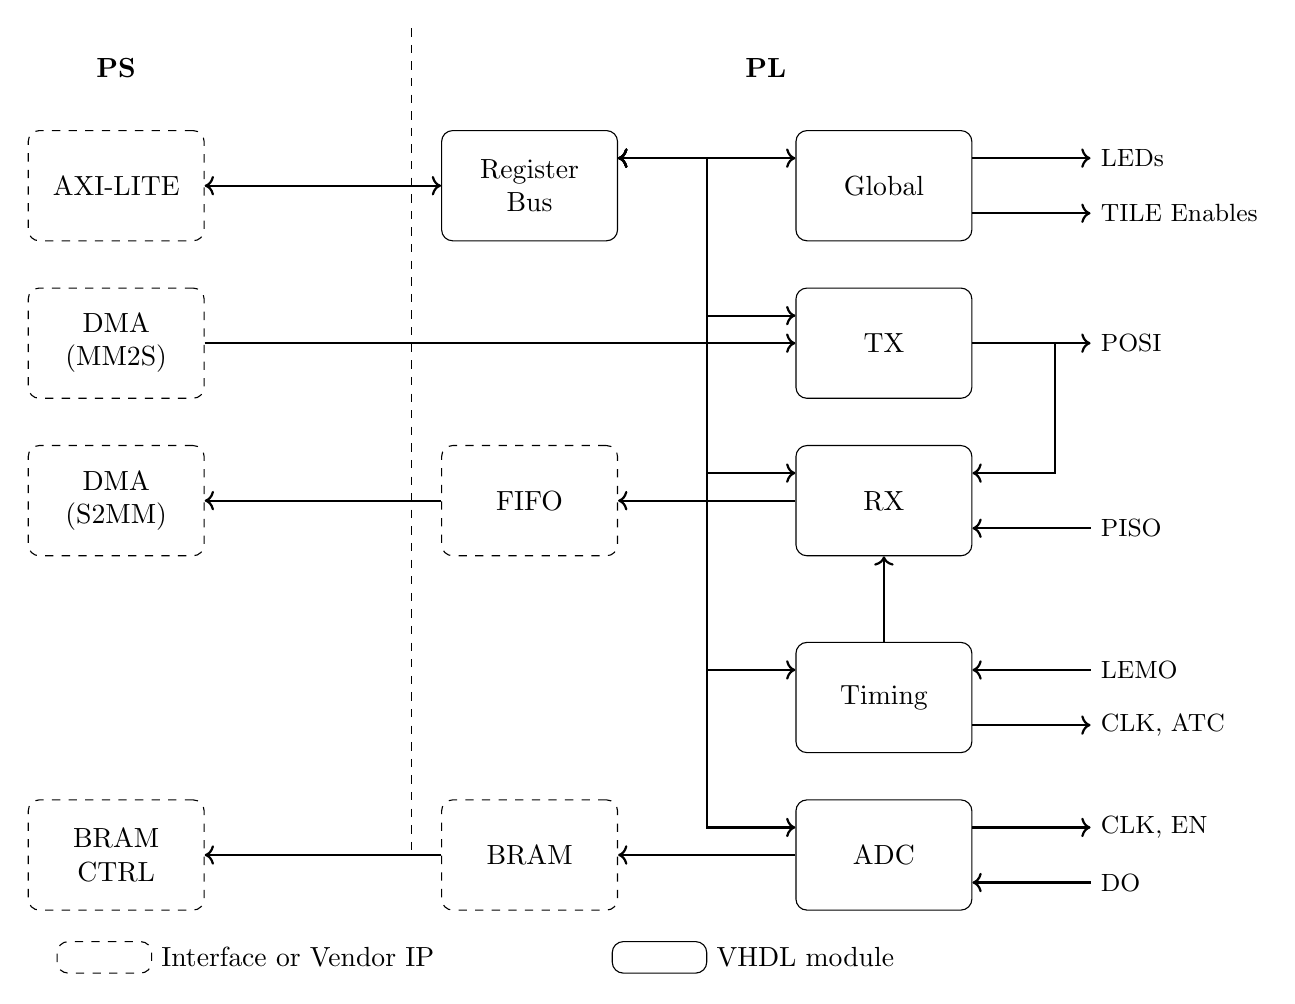
\begin{tikzpicture}[x=1.5cm, y=1cm]

% Dashed vertical separator between columns 1 and 2 at x = 2.5
\draw[dashed] (3.5,10.5) -- (3.5,0);
\node at (1.0,10) {\textbf{PS}};
\node at (6.5,10) {\textbf{PL}};

% Uniform box size
\def\boxwidth{2.0cm}
\def\boxheight{1.4cm}

% PS column (x ≈ 1) - align with first three boxes in PL column, uniform spacing 1.75 units
\node[draw, rounded corners, dashed, minimum width=\boxwidth, minimum height=\boxheight, text width=\boxwidth, align=center] (axi)  at (1,8.5) {AXI-LITE};
\node[draw, rounded corners, dashed, minimum width=\boxwidth, minimum height=\boxheight, text width=\boxwidth, align=center] (mm2s) at (1,6.5) {DMA\\(MM2S)};
\node[draw, rounded corners, dashed, minimum width=\boxwidth, minimum height=\boxheight, text width=\boxwidth, align=center] (s2mm) at (1,4.5)  {DMA\\(S2MM)};
\node[draw, rounded corners, dashed, minimum width=\boxwidth, minimum height=\boxheight, text width=\boxwidth, align=center] (bramc) at (1,0.0)  {BRAM\\CTRL};

% Center column (x ≈ 4.5)
\node[draw, rounded corners, minimum width=\boxwidth, minimum height=\boxheight, text width=\boxwidth, align=center] (fanout) at (4.5,8.5) {Register\\Bus};
\node[draw, rounded corners, dashed, minimum width=\boxwidth, minimum height=\boxheight, text width=\boxwidth, align=center] (fifo) at (4.5,4.5) {FIFO};
\node[draw, rounded corners, dashed, minimum width=\boxwidth, minimum height=\boxheight, text width=\boxwidth, align=center] (bram) at (4.5,0.0)  {BRAM};


% PL column (x ≈ 7.5) - align first three boxes vertically with PS column
\node[draw, rounded corners, minimum width=\boxwidth, minimum height=\boxheight, text width=\boxwidth, align=center] (global) at (7.5,8.5) {Global};
\node[draw, rounded corners, minimum width=\boxwidth, minimum height=\boxheight, text width=\boxwidth, align=center] (tx)     at (7.5,6.5) {TX};
\node[draw, rounded corners, minimum width=\boxwidth, minimum height=\boxheight, text width=\boxwidth, align=center] (rx)     at (7.5,4.5) {RX};
\node[draw, rounded corners, minimum width=\boxwidth, minimum height=\boxheight, text width=\boxwidth, align=center] (timing) at (7.5,2.0) {Timing};
\node[draw, rounded corners, minimum width=\boxwidth, minimum height=\boxheight, text width=\boxwidth, align=center] (adc)    at (7.5,0.0) {ADC};

% PS/IP Interface Arrows
\draw[->, thick] (rx.west) -- (fifo.east);
\draw[->, thick] (fifo.west) -- (s2mm.east);
\draw[<->, thick] (axi.east) -- (fanout.west);
\draw[->, thick] (adc.west) -- (bram.east);
\draw[->, thick] (bram.west) -- (bramc.east);

% timestamp:
\draw[->, thick] (timing.north) -- (rx.south);

% REGBUS arrows:
\draw[<->, thick] ($(fanout.east)+(0,0.35cm)$) -- ++(0.75,0) -- ($(global.west)+(0,0.35cm)$);
\draw[<->, thick] ($(fanout.east)+(0,0.35cm)$) -- ++(0.75,0) -- ++(0,-2) -- ($(tx.west)+(0,0.35cm)$);
\draw[<->, thick] ($(fanout.east)+(0,0.35cm)$) -- ++(0.75,0) -- ++(0,-4) -- ($(rx.west)+(0,0.35cm)$);
\draw[<->, thick] ($(fanout.east)+(0,0.35cm)$) -- ++(0.75,0) -- ++(0,-6.5) -- ($(timing.west)+(0,0.35cm)$);
\draw[<->, thick] ($(fanout.east)+(0,0.35cm)$) -- ++(0.75,0) -- ++(0,-8.5) -- ($(adc.west)+(0,0.35cm)$);

\draw[->, thick] (mm2s.east) -- ++(1,0) -- ++(0,0) -- (tx.west);


% Draw arrow from 'global' node east side to right, with label
\draw[->, thick] ($(global.east)+(0,0.35cm)$) -- ++(1.0,0) node[anchor=west, font=\small] {LEDs};
\draw[->, thick] ($(global.east)-(0,0.35cm)$) -- ++(1.0,0) node[anchor=west, font=\small] {TILE Enables};

\draw[->, thick] ($(tx.east)+(0,0.00cm)$) -- ++(1.0,0) node[anchor=west, font=\small] {POSI};
\draw[->, thick] ($(tx.east)+(0,0.00cm)$) -- ++(0.7,0) -- ++(0,-1.65) -- ++(-0.7,0);

\draw[<-, thick] ($(rx.east)-(0,0.35cm)$) -- ++(1.0,0) node[anchor=west, font=\small] {PISO};

\draw[<-, thick] ($(timing.east)+(0,0.35cm)$) -- ++(1.0,0) node[anchor=west, font=\small] {LEMO};
\draw[->, thick] ($(timing.east)-(0,0.35cm)$) -- ++(1.0,0) node[anchor=west, font=\small] {CLK, ATC};

\draw[->, thick] ($(adc.east)+(0,0.35cm)$) -- ++(1.0,0) node[anchor=west, font=\small] {CLK, EN};
\draw[<-, thick] ($(adc.east)-(0,0.35cm)$) -- ++(1.0,0) node[anchor=west, font=\small] {DO};



% Legend
\begin{scope}[shift={(0,-1.5)}] % adjust this shift to position the legend
  \draw[dashed, rounded corners] (0.5,0.0) rectangle ++(0.8,0.4);
  \node[anchor=west] at (1.3,0.2) {Interface or Vendor IP};

  \draw[rounded corners] (5.2,0.0) rectangle ++(0.8,0.4);
  \node[anchor=west] at (6.0,0.2) {VHDL module};
\end{scope}

\end{tikzpicture}
\caption{Top-Level Block Diagram of HW Demonstration Firmware}
\label{fig:pl-top}
\end{figure}

\noindent
Both vendor IP and standard interfaces are featured prominantly in the design:
\begin{itemize}
 \item AXI-Lite (relatively slow 32-bit transfers) is used for custom registers.
 \item DMA (high peformance direct memory access) is used for high-bandwith TX and RX transfers.
 \item A AXI Stream FIFO is used to buffer the RX data between the RX unit and the DMA engine.
 \item BRAM (Block RAM) is used by the ADC unit to store the time series of conversion data.
\end{itemize}
The AXI interface is widely used throughout the design, and is well
documented elsewhere.  A critical point for understanding the AXI
protocol is that data is transfered from a data producer to a data
consumer when and only when a beat occurs.  {\bf A beat is defined as
  a clock-cycle during which the data producer asserts its valid
  signal and the data consumer asserts a busy signal.}
There are further
requirements, but this is sufficient to understand basic operation.
For convenience, we use the same valid and ready handshake elsewhere
in the design, even when we do not implement an AXI interface.
The design uses one custom interface: the register bus (REGBUS).  Each
unit-level module is a secondary on the REGBUS, and is guaranteed to
respond on the clock cycle immediately following a read or write
request from the REGBUS primary.  The PS drivers access the REGBUS
interface via AXI-Lite.

\begin{figure}[htbp]
  \centering
  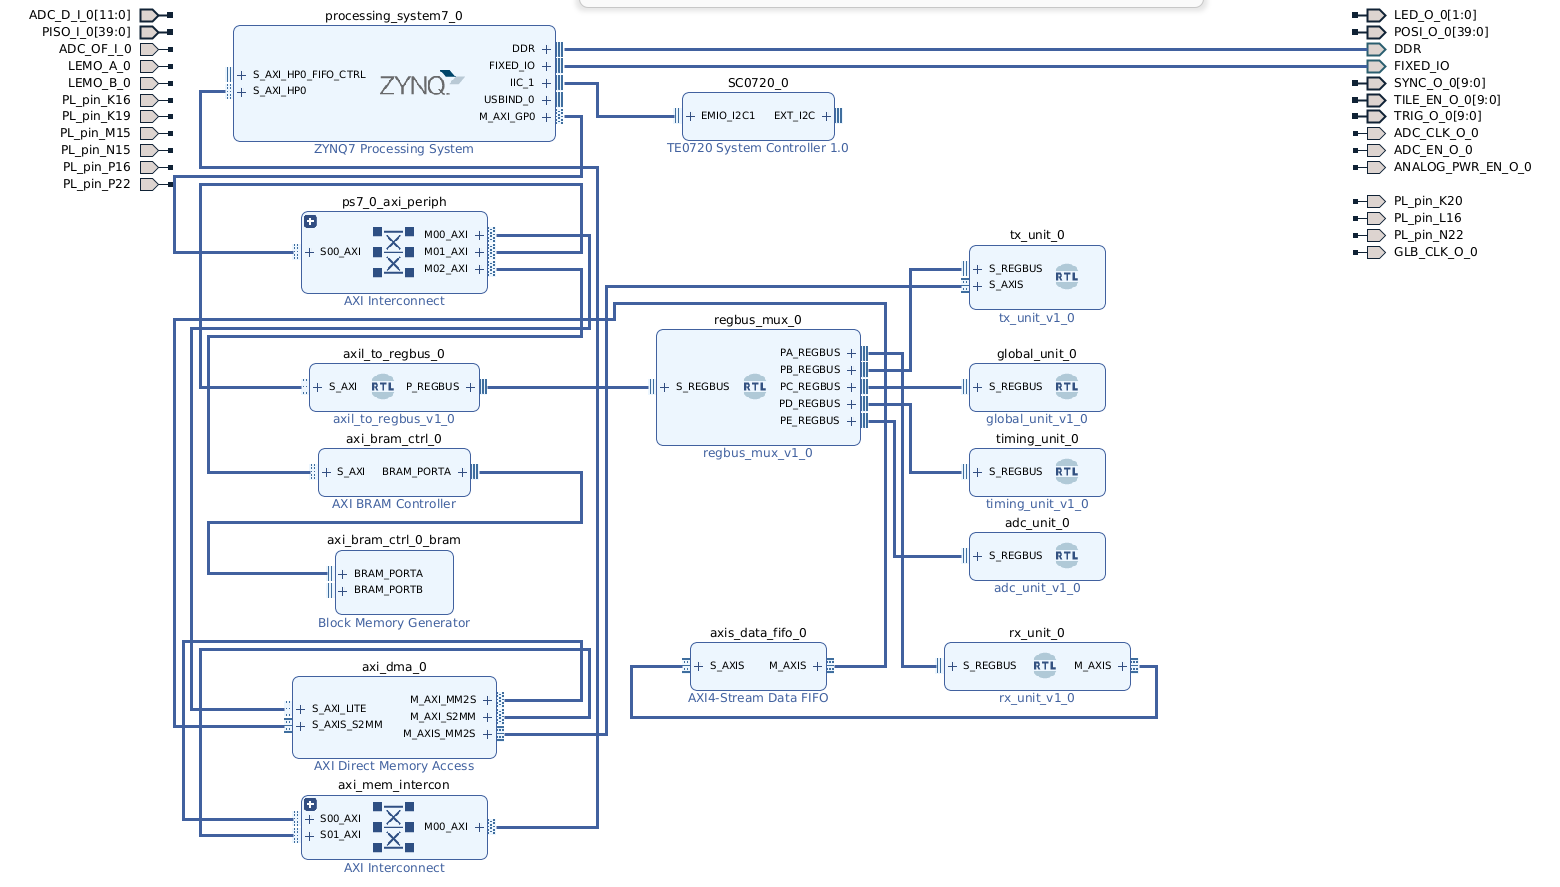
\includegraphics[angle=90, width=\paperheight, height=\paperwidth, keepaspectratio]{figs/pacman-top.png}
\caption{Vivado Block Design (Interfaces View) }
\label{fig:vivado-top}
\end{figure}



\subsection{Registers}


\begin{figure}[htbp]
  \centering
  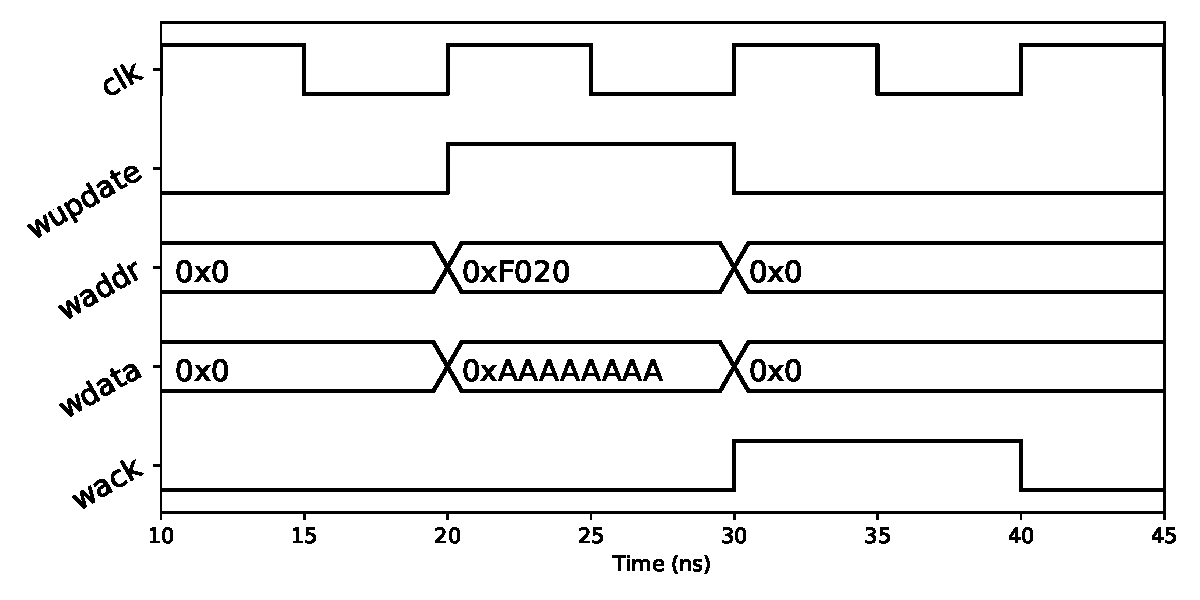
\includegraphics[width=0.68\paperwidth, keepaspectratio]{timing_diagrams/single_write.pdf}
\caption{Single REGBUS write request (output of ghdl testbench)}
\label{fig:single-read}
\end{figure}

Access to registers in the PL firmware is done via a simple custom
register bus (REGBUS).

A REGBUS write request is made by the single primary setting the
16-bit write address to that of the register of interest, the 32-bits
of write data to the desired value, and the write update bit high.
The secondary on the bus responsible for that register responds on the
next clock cycle by setting the write acknowledge bit high and
performing any other desired effect, such as setting a register to the
value of the write data.  A single write request is illustrated in
Fig.~\ref{fig:single-write}.  Command registers are implemented by
setting a command signal high for one clock cycle after a write to the
command register address, often ignoring the write data entirely.

\begin{figure}[htbp]
  \centering
  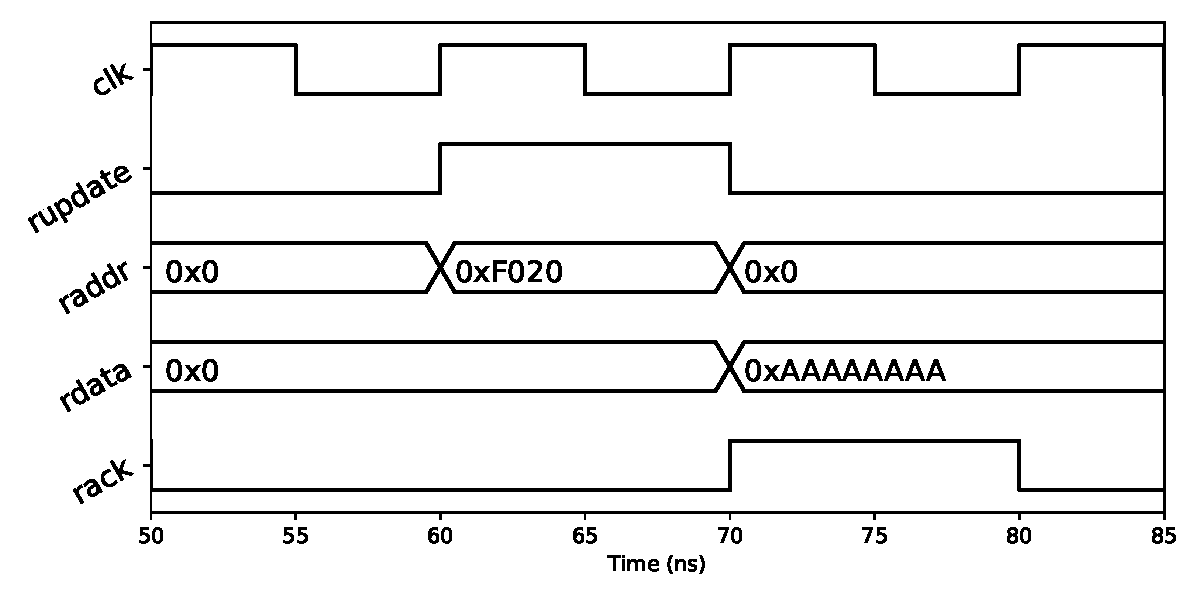
\includegraphics[width=0.68\paperwidth, keepaspectratio]{timing_diagrams/single_read.pdf}
\caption{Single REGBUS read request (output of ghdl testbench)}
\label{fig:single-read}
\end{figure}

A read request on the bus is made by the single primary setting the
16-bit read address to that of the register of interest and setting
the read update bit high.  The secondary on the bus responsible for
that register responds on the next clock cycle by setting the 32-bit
read data to the value associated with the register of interest, and
setting the read acknowledge bit high.  A single read request is illustrated in
Fig.~\ref{fig:single-read}.

The register bus is implemented by a module ({\tt axil\_to\_regbus.vhd})
which translates AXI-Lite requests from the PS to read and write
requests on the REGBUS.  Because FPGAs do not have internal tristate
buffers, the bus implementation also requires a multiplexer {\tt
  regbus\_mux.vhd} to connect the REBGUS primary to multiple
secondaries.

The 16-bit address space for PACMAN registers is allocated in a
hierachical fashion, represented as
$$0{\rm x}SRRR$$
with the most significant four bits $0{\rm x}S$ defining the scope, and the
remaining 12 bits $0{\rm x}RRR$ defining the specific register within the scope.
For example, the scratch A register (0x020), of the global unit (0xF)
would be found at the 32-bit address:
$$0{\rm xF}020.$$
The scopes are allocated as shown in Table~\ref{tbl:scope}.
\begin{table}
\caption{\label{tbl:scope} The most significant four bits of the register address, referred to as the scope, is allocated as shown.}
\begin{center}
\begin{tabular}{|lll|}
\hline
Scope      & Hexadecimal & Binary \\
\hline
Global     & 0{\rm x}F         & 0b1111 \\
Timing     & 0{\rm x}E         & 0b1110 \\
ADC        & 0{\rm x}D         & 0b1101 \\
TX         & 0{\rm x}4-0{\rm x}7     & 0b01XX \\
RX         & 0{\rm x}0-0{\rm x}3     & 0b00XX \\
(Reserved) & 0{\rm x}8-0{\rm x}C     & 0b1000-0b1100 \\
\hline
\end{tabular} \\
\end{center}
\end{table}
The RX and TX unit are allocated a range of scopes to more readily
accommodate the large number of registers associated with all 40 uarts
(e.g. lost packet counts per uart channel).  Further discussion of
PACMAN registers is left to the subsections for each unit.

\subsection{Global Unit}

\begin{table}
\label{tbl:global-reg}
\caption{Registers managed by the global unit}
\begin{center}
\begin{tabular}{|lll|}
\hline
Register    & Address & RO/RW \\
\hline
STATUS      & 0xF000 & RO \\
ENABLES     & 0xF010 & RW \\
LEDS        & 0xF014 & RW \\
SCRATCH\_A  & 0xF020 & RW \\
SCRATCH\_B  & 0xF024 & RW \\
FIRMWARE\_MAJOR   & 0xFF10 & RO \\
FIRMWARE\_MINOR   & 0xFF14 & RO \\
FIRMWARE\_LETTER  & 0xFF18 & RO \\
HARDWARE\_MAJOR   & 0xFF20 & RO \\
HARDWARE\_MINOR   & 0xFF24 & RO \\
HARDWARE\_LETTER  & 0xFF28 & RO \\
SYNTHESIS\_DATE   & 0xFF30 & RO \\
GIT\_HASH\_UPPER   & 0xFF40 & RO \\
GIT\_HASH\_LOWER   & 0xFF44 & RO \\
VIVADO\_MAJOR     & 0xFF50 & RO \\
VIVADO\_MINOR     & 0xFF54 & RO \\
\hline
\end{tabular}
\end{center}
\end{table}

\begin{table}
\caption{\label{tbl:global-bit-fields} Bit fields:  discription }
\begin{center}
\begin{tabular}{|llll|}
\hline
Register & Field             & Bits & Mask       \\
\hline
ENABLES  & TILE\_ENABLES       & 0-9  & 0x000003FF \\
         & TILE\_POWER\_ENABLE &  16  & 0x00010000 \\
\hline
LEDS     & LED\_3              & 0    & 0x00000001 \\
         & LED\_4              & 1    & 0x00000002 \\
\hline
\end{tabular}
\end{center}
\end{table}

The global unit handles simple board-wide tasks, and manages the
registers listed in Table~\ref{tbl:global-reg}.  The bit field
interpretations for some registers are shown in
Table~\ref{tbl:global-bit-fields}.  The read-only firmware registers
can be used to determine the firmware version installed, and the
read-only hardware registers can be used to check the hardware version
for which the firmware was built.  The FIRMWARE\_BUILD and HARDWARE\_BUILD registers are reserved.
The read-write scratch registers SCRATCH\_A and SCRATCH\_B
have no impact beyond storing and retrieving the register value, and
are useful for testing the operation of the AXI-Lite and REGBUS
interfaces.

Providing power and data I/O to the TILES requires enabling power to
the tile power subsystem (called ANALOG\_POWER\_ENABLE in hardware
schematics) as well as enabling the individual tile.  These settings
are available in the ENABLES register, using the bit fields
TILE\_POWER\_ENABLE and TILE\_ENABLES.  While a tile is disabled, even with
tile power enabled, the LVDS transmitters and receivers will be off,
and both VDDD and VDDA are at zero.  Setting the values of VDDD and
VDDDA, and monitoring currents and voltages on the board, is done over
I2C, by the PS, and so is not part of the PL firmware design.

The PACMAN has two LEDs controlled by the PL.  Their behavior is
controlled by the LEDS register.  In the current iteration, each LED
is simply turned on or off directly, by the LED\_3 and LED\_4 bits,
but in the future, they could be driven by specific conditions as
well.  Two additional LEDs are driven from the PS, and are not part of
the PL firmware design.  Two LEDs on the Trenz module are also
controllable from the PS.  The global unit also provides a global
status register (STATUS).  In the current implementation, this
register is implemented as a fixed pattern.

\subsection{TX Unit}

\begin{figure}[htbp]
\centering
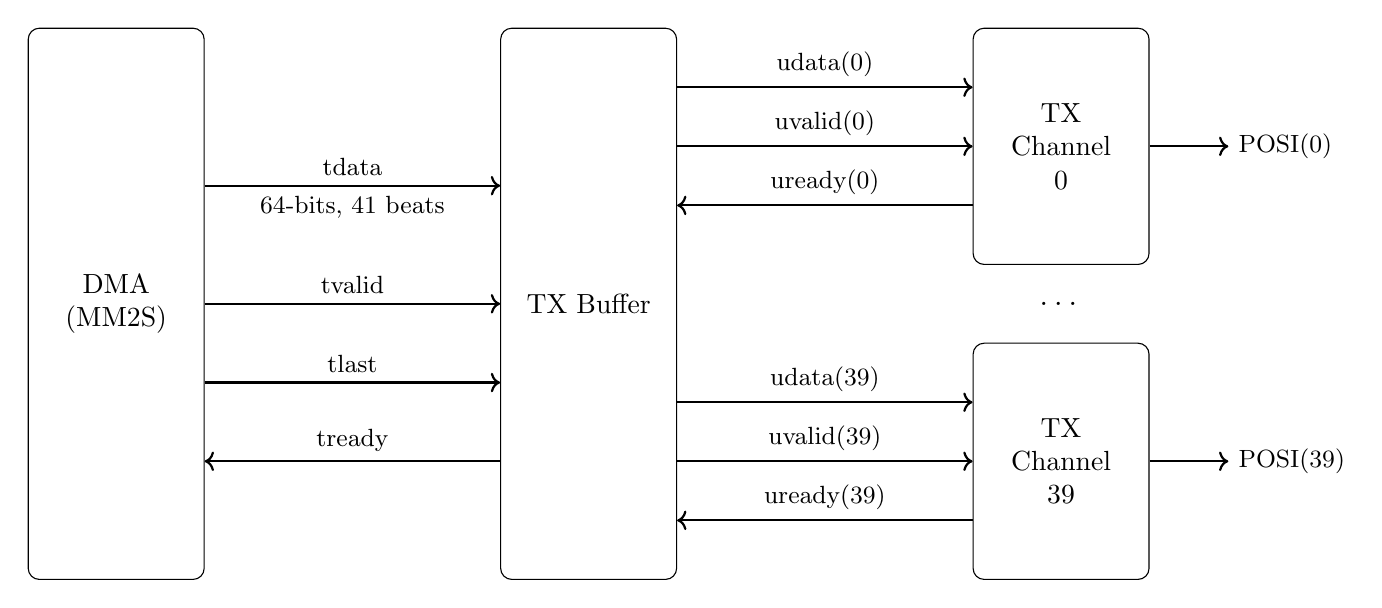
\begin{tikzpicture}[x=1cm, y=1cm]

% Uniform box size
\def\boxwidth{2.0cm}
\def\boxshort{3.0cm}
\def\boxtall{7.0cm}

\node[draw, rounded corners, minimum width=\boxwidth, minimum height=\boxtall, text width=\boxwidth, align=center] (mm2s) at (1,3) {DMA\\(MM2S)};
\node[draw, rounded corners, minimum width=\boxwidth, minimum height=\boxtall, text width=\boxwidth, align=center] (tx)   at (7,3) {TX Buffer};

\node[draw, rounded corners, minimum width=\boxwidth, minimum height=\boxshort, text width=\boxwidth, align=center] (a)   at (13,5) {TX \\ Channel \\ 0};
\node[draw, rounded corners, minimum width=\boxwidth, minimum height=\boxshort, text width=\boxwidth, align=center] (b)   at (13,1) {TX \\ Channel \\ 39};

\node at (13,3) {\large\textellipsis};

\coordinate (aa) at ($(a.west)+(0,0.75)$);
\coordinate (ab) at ($(a.west)+(0,0.00)$);
\coordinate (ac) at ($(a.west)-(0,0.75)$);
\draw[->, thick] (tx.east |- aa) -- node[above, font=\small] {udata(0)} (aa);
\draw[->, thick] (tx.east |- ab) -- node[above, font=\small] {uvalid(0)} (ab);
\draw[<-, thick] (tx.east |- ac) -- node[above, font=\small] {uready(0)} (ac);

\coordinate (ba) at ($(b.west)+(0,0.75)$);
\coordinate (bb) at ($(b.west)+(0,0.00)$);
\coordinate (bc) at ($(b.west)-(0,0.75)$);
\draw[->, thick] (tx.east |- ba) -- node[above, font=\small] {udata(39)} (ba);
\draw[->, thick] (tx.east |- bb) -- node[above, font=\small] {uvalid(39)} (bb);
\draw[<-, thick] (tx.east |- bc) -- node[above, font=\small] {uready(39)} (bc);


% Stream Interface Arrows
\draw[->, thick]
  ($(mm2s.east)+(0,1.5)$)
  -- node[above, font=\small] {tdata}
     node[below, font=\small] {64-bits, 41 beats}
  ($(tx.west)+(0,1.5)$);
\draw[->, thick] ($(mm2s.east)+(0,0.0)$) -- node[above, font=\small] {tvalid} ($(tx.west)+(0,0.0)$);
\draw[->, thick] ($(mm2s.east)-(0,1.0)$) -- node[above, font=\small] {tlast} ($(tx.west)-(0,1.0)$);
\draw[<-, thick] ($(mm2s.east)-(0,2.0)$) -- node[above, font=\small] {tready} ($(tx.west)-(0,2.0)$);

% POSI Output
\draw[->, thick] (a.east) -- ++(1.0,0) node[anchor=west, font=\small] {POSI(0)};
\draw[->, thick] (b.east) -- ++(1.0,0) node[anchor=west, font=\small] {POSI(39)};


\end{tikzpicture}
\caption{Data path in the TX Unit}
\label{fig:tx-unit}
\end{figure}

\noindent
The TX unit is responsible for configuration, operation, and
monitoring of transmission to the tile cards via 40 uart channels.  A
block diagram of the TX unit is shown in Fig.~\ref{fig:tx-unit}.  The
data to be transmitted arrives as an AXI stream, which is filled by
the PS using DMA.

\begin{table}[htbp]
\label{tbl:tx-dma}
\caption{Contents of the TX DMA packet}
\begin{center}
\begin{tabular}{|lll|}
\hline
Beat: & Contents: & Description \\
\hline
1     & {\tt 0}x{\tt 000000MMMMMMMMMM} & M=UART Mask \\
2     & {\tt 0}x{\tt AAAAAAAABBBBBBBB} & A=UART[1], B=UART[0]   \\
3     & {\tt 0}x{\tt AAAAAAAABBBBBBBB} & A=UART[3], B=UART[2]   \\
      & $\ldots$           &                        \\
21    & {\tt 0}x{\tt AAAAAAAABBBBBBBB} & A=UART[39], B=UART[38] \\
\hline
\end{tabular}
\end{center}
\end{table}

The TX Buffer sub-module contains a single buffer which holds incoming
stream data until a complete DMA packet has been received.  As shown
in Table~\ref{tbl:tx-dma}, a complete DMA packet consists of a 128-bit
header and 20 128-bit words.  The header contains a channel mask
specifying which channels have data to transmit.  The 20 128-bit words
contain 40 uart payloads, each of 64 bits.  The DMA packet is the same
size independent of how many UARTs are activated by the mask.
Payloads from inactive UARTs are simply ignored.

\begin{figure}[htbp]
  \centering
  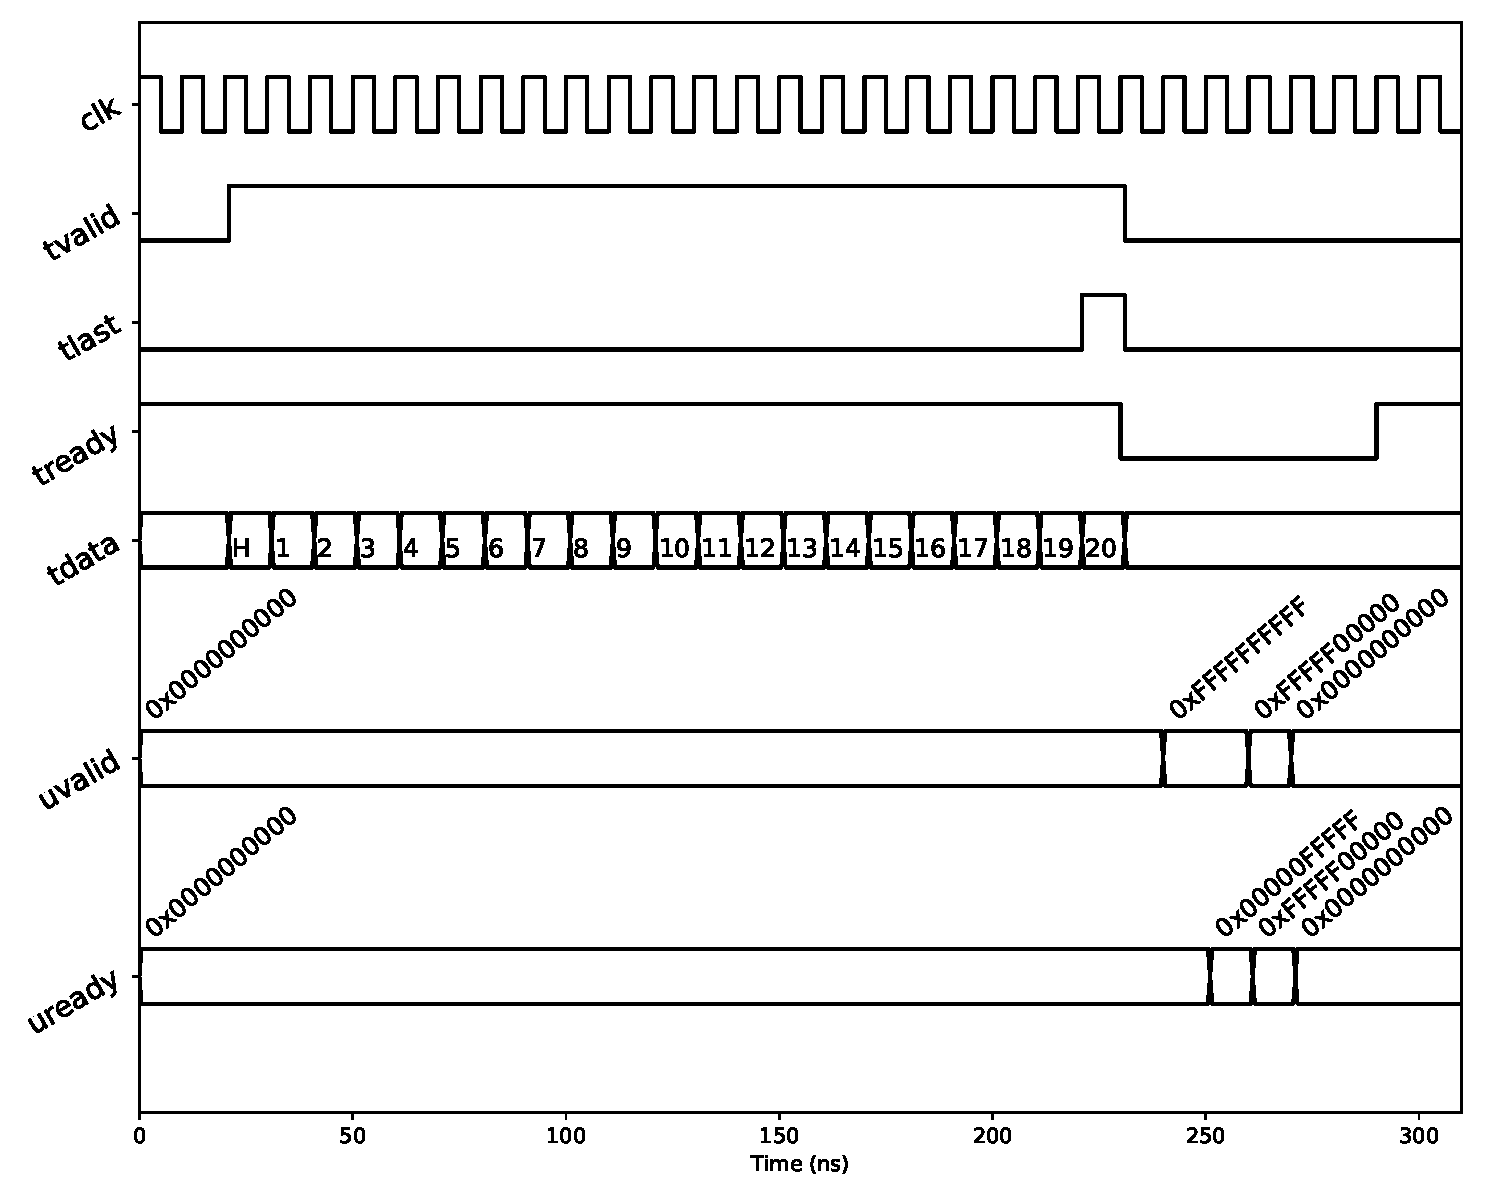
\includegraphics[width=0.85\paperwidth, keepaspectratio]{timing_diagrams/tx_buffer.pdf}
\caption{TX buffer handling a single DMA packet (output of ghdl testbench)}
\label{fig:tx-buffer}
\end{figure}

A timing diagram of the TX Buffer handling a single DMA packet is
presented in Fig.~\ref{fig:tx-buffer}.  As discussed in the
introduction, the AXI interface transfers data from producer to
consumer when and only when both valid and ready are asserted on the
same clock-cycle, called a beat.  At the start, the TX buffer is
empty, and so the stream ready ({\tt tready}) signal is asserted by TX
buffer.  When data is available via DMA, the AXI stream asserts stream
valid ({\tt tvalid}).  This continues for 21 beats.  During the last
beat, the stream asserts the last signal ({\tt tlast}) indicating the
end of the packet.  The TX buffer will now contain a complete DMA
packet, and so the TX buffer deasserts stream ready ({\tt tready})
which halts the stream.

The UART transmission is handled by 40 instances of the TX Channel
sub-module, with one assigned to each UART channel.  Even though this
stage is not an AXI interface, the valid and ready handshake is used
again, this time with one handshake per UART channel.  The TX buffer
asserts a valid signal ({\tt uvalid(i)}) for each UART channel that
has data available, as specified in the mask located in the DMA packet
header.  Assuming a TX channel is not currently transmitting, it
loads valid data presented by TX buffer into its internal shift registers for
transmission, and asserts ready ({\tt uready(i)}) on the next clock cycle.

Upon detecting a beat, the UART valid signal for the channel is
cleared on the next clock cycle, indicating the data for that channel
has been transferred to the shift register of the corresponding TX
channel for transmission.  When and only when all UART valid signals
are cleared, the buffer is empty, the TX buffer asserts stream ready
({\tt tready}) and, assuming data is available via DMA, the cycle
begins again.

The slowest component in this chain is the UART transmission, which is
bit serial.  At 10 MHz, transmitting 64 bits, plus a start and stop
bit, requires 660 100 MHz clock cycles.  The DMA transfer of a single
packet takes only 21 clock cycles\footnote{This is why we opt for a
simple fixed length transmission, there is nothing further to be
gained by e.g. zero suppression.}  While each TX channel is
transmitting, it deasserts its ready, which prevents a beat with TX
Buffer, and causes TX Buffer to deassert stream ready once it has a
DMA packet buffered.  As soon as the current transmission is complete,
the next transmission begins immediately.  As long as new data is
available via DMA, the transmitters run flat out.  However, a configurable
parameter inserts an artificial delay between each transmission cycle,
which allows the TX speed to be throttled as needed to avoid
overwhelming the ASICs.

You might notice in Fig.~\ref{fig:tx-buffer} that the timing in TX
buffer is not particularly tight.  The UART valid signals ({\tt
  uvalid(i)}) and the Stream ready ({\tt tready}) could in principle
all go high one clock cycle earlier.  The additional delay is due to
pipelined logic.  The AXI stream delivers the UART data with UARTs
handled serially (two at a time).  An initial stream reader stage
parallizes the stream data, and registers its output.  Likewise, the
calculation of the logical or across all of the UART valid signals
({\tt uvalid(i)}) is registered as well.  These calculations could be
made combinatoric if tighter timing was needed.  However, as discussed
above, TX buffer is more than fast enough to keep up with the UART
transmission at full speed, so we prefer the added robustness of the
pipelined calculation.

The UART modules have been left unchanged from the legacy firmware.
It was an intentional design choice to leave the PACMAN interfaces (to
the ASICs, and to DAQ via pacman-server) unchanged during the initial
development of the the 3.X firmware, so that it could proceed without
the need for extensive testing on ASICs and without any changes to the
DAQ.  The legacy UART design includes an unnecessary pause between
start and stop bits, which increases the transmission time to 670
clock cycles (at 10 MHz).  Unlike the TX buffer latency, this is at
the timing bottle neck for the entire TX unit.  However, this is still
not problematic, because, as discussed above, we throttle down the TX
transmission rate to avoid overwhelming the ASICs.  An update to the
UART firmware is planned for a future firmware release, but only after
we have an extensive testbench available using actual ASICs.

\begin{table}
\caption{\label{tbl:tx-scope} All TX registers have leading two bits 0, and the next six bits define the channel.  That least significant byte (XX below) specifies the register.}
\begin{center}
\begin{tabular}{|lll|}
\hline
Channel      & $C$                   & TX Register Address          \\
\hline
UART 0-39    & 0{\rm x}00-0{\rm x}27 & 0{\rm x}00XX-0{\rm x}27XX \\
Broadcast    & 0{\rm x}3B            & 0{\rm x}3BXX              \\
In Common    & 0{\rm x}3F            & 0{\rm x}3FXX              \\
\hline
\end{tabular}
\end{center}
\end{table}

Configuration and monitoring of the TX unit is performed over the
AXI-LITE to REGBUS interface.  Recall that the first four bits of the
32-bit address space is referred to as the scope, and is used to
divide the 16-bit address space between different units.  The TX unit
is allocated the range of scopes from 0x0 to 0x3.  Consistent with
this assignment, the the most significant bytes of a TX register
address are interpreted as:
$${\rm 0b00}cc cccc$$
where
$$C \equiv 0{\rm b}cccccc$$ is the UART channel, taking values from 0
to 63.  In addition to the 40 physical UART channels, assigned
channels 0 to 39 (0x00 to 0x27), there are two notional channels:
broadcast (0x3B) and in common (0x3F).  This is summarized in Table~\ref{tbl:tx-scope}.
A single write to a UART register at the broadcast channel sets that
registers for {\bf all} UARTs to the specified value.  Attempting to
read from the broadcast channel is invalid.  Registers associated to
the entire TX unit are assigned to the notional channel ``in common''.
Both read and write to the common channel, for defined common
registers, is valid.


\begin{table}
\label{tbl:tx-reg}
\caption{Registers managed by the TX unit}
\begin{center}
\begin{tabular}{|llll|}
\hline
Register    & Address   & RWC & Per UART    \\
\hline
UART\_STATUS     & 0x00  & RO  & Per UART   \\
UART\_CONFIG     & 0x04  & RW  & Per UART   \\
UART\_LOOK\_C    & 0x18  & RO  & Per UART   \\
UART\_LOOK\_D    & 0x1C  & RO  & Per UART   \\
UART\_STARTS     & 0x20  & RO  & Per UART   \\
UART\_BEATS      & 0x24  & RO  & Per UART   \\
UART\_CHAN       & 0x50  & RO  & Per UART   \\
BUFFER\_STATUS     & 0xA0  & RO  & In Common  \\
ZERO\_CNTS       & 0xA8  & CMD & In Common  \\
\hline
\end{tabular}
\end{center}
\end{table}

\begin{table}
\label{tbl:tx-bit-fields}
\caption{Bit field descriptions for TX register}
\begin{center}
\begin{tabular}{|llll|}
\hline
Register & Field    & Bits & Mask       \\
\hline
UART\_STATUS  & (Expert)   & 31-0  & {\tt 0}x{\tt FFFFFFFF}  \\
\hline
UART\_CONFIG  & RATIO      & 7-0   & {\tt 0}x{\tt 000000FF}  \\
              & PHASE      & 11-8  & {\tt 0}x{\tt 00000F00}  \\
              & MODE       & 13-12 & {\tt 0}x{\tt 00003000}  \\
              & (Reserved) & 15-14 & {\tt 0}x{\tt 0000C000}  \\
              & DELAY      & 31-16 & {\tt 0}x{\tt FFFF0000}  \\
\hline
BUFFER\_STATUS  & (Expert)   & 31-0  & {\tt 0}x{\tt FFFFFFFF}  \\
\hline
\end{tabular}
\end{center}
\end{table}

The registers managed by the TX unit are presented in
Table~\ref{tbl:tx-reg}, and bit field interpretations for some of the
registers are provided in Table~\ref{tbl:tx-bit-fields}. The UART
configuration (UART\_CONFIG) includes fields for a phase offset (in 10 ns
ticks) and a clock divider (slow down factor) of the TX UART clock
relative to the 100 ns clock sent directly to the ASICs.  Normal
operation is mode=1.  For mode=0, the TX UART is off, and the channel
holds ready high.  The upper 16 bits of the register is the
configurable delay (in 10 ns ticks) inserted between TX cycles.  The
UART status registers (UART\_STATUS, one per UART) and TX buffer status
(BUFFER\_STATUS) interpretation is currently expert only, and not documented
here, but the counts (explained below).  More user friendly
quantities (derived from the status registers) are available and
described below.

The look registers (UART\_LOOK\_C and UART\_LOOK\_D) are the least significant
and most significant 32-bit words from the most recent transmission
request sent to each UART channel.  These buffers are used to verify
the operation of the DMA to UART channel transmission, and do not test
the actual operation of the UART transmitter.  Operation of the UART
itself can be verified by software loopback of the UART output to the
RX UARTs (as described in the RX section) or by physical loopback.
The number of beats encountered (UART\_BEATS) and the number of
transmission start bits sent (UART\_STARTS) is available for each UART.
These counts are cleared upon reset and by writing the zero counts
(ZERO\_CNTS) register.


The TX firmware has been demonstrated in the hardware (using both
bare-metal applications and Linux) to run continuously at maximum
speed without any bit errors.

\newpage
\subsection{RX Unit}

\begin{figure}[htbp]
\centering
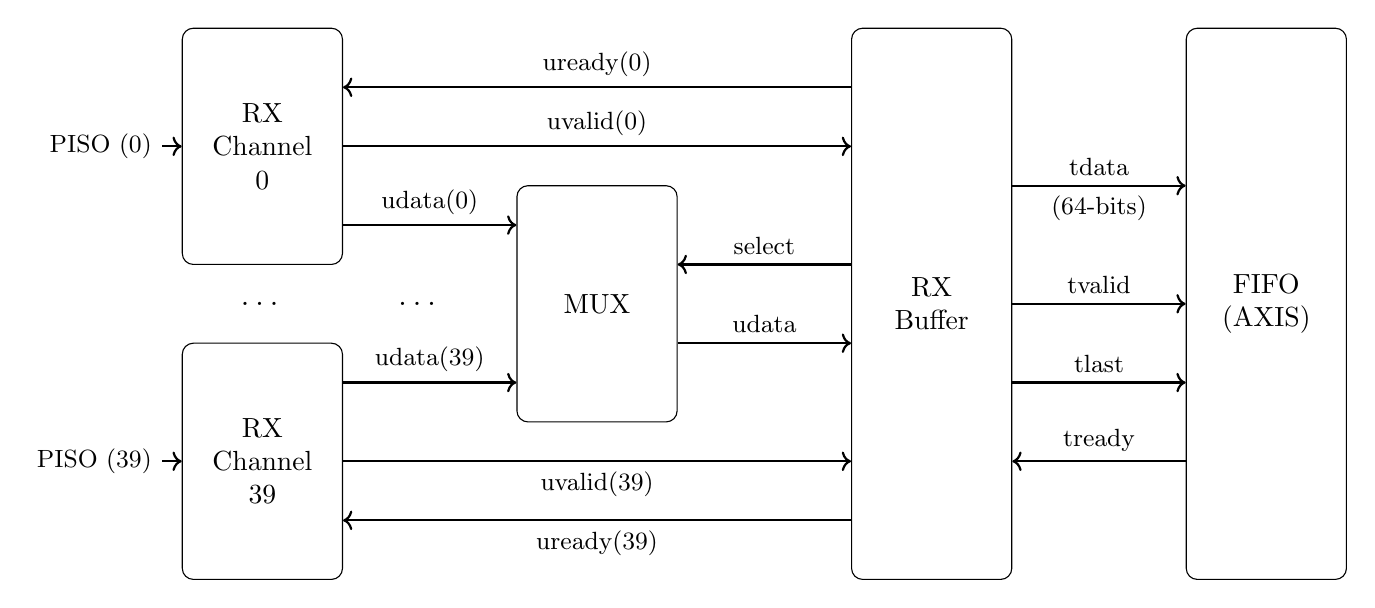
\begin{tikzpicture}[x=1cm, y=1cm]

% Uniform box size

\def\boxwidth{1.8cm}
\def\boxshort{3cm}
\def\boxmed{3.5cm}
\def\boxtall{7.0cm}

\node[draw, rounded corners, minimum width=\boxwidth, minimum height=\boxshort, text width=\boxwidth, align=center]
(a)    at (0,5)  {RX \\ Channel \\ 0};
\node[draw, rounded corners, minimum width=\boxwidth, minimum height=\boxshort, text width=\boxwidth, align=center]
(b)    at (0,1)  {RX \\ Channel \\ 39};
\node[draw, rounded corners, minimum width=\boxwidth, minimum height=\boxshort,  text width=\boxwidth, align=center]
(mux)  at (4.25,3)  {MUX};
\node[draw, rounded corners, minimum width=\boxwidth, minimum height=\boxtall,  text width=\boxwidth, align=center]
(buf)  at (8.5,3)  {RX \\ Buffer};
\node[draw, rounded corners, minimum width=\boxwidth, minimum height=\boxtall,  text width=\boxwidth, align=center]
(fifo) at (12.75,3) {FIFO\\(AXIS)};

\node at (0,3) {\large\textellipsis};

\node at (2,3) {\large\textellipsis};  

\coordinate (aa) at ($(a.east)+(0,0.75)$);
\coordinate (ab) at ($(a.east)+(0,0.00)$);
\coordinate (ac) at ($(a.east)-(0,1.00)$);
\draw[->, thick] (buf.west |- aa) -- node[above, font=\small] {uready(0)} (aa);
\draw[<-, thick] (buf.west |- ab) -- node[above, font=\small] {uvalid(0)} (ab);
\draw[<-, thick] (mux.west |- ac) -- node[above, font=\small] {udata(0)} (ac);

\coordinate (ba) at ($(b.east)+(0,1.00)$);
\coordinate (bb) at ($(b.east)+(0,0.00)$);
\coordinate (bc) at ($(b.east)-(0,0.75)$);
\draw[<-, thick] (mux.west |- ba) -- node[above, font=\small] {udata(39)} (ba);
\draw[<-, thick] (buf.west |- bb) -- node[below, font=\small] {uvalid(39)} (bb);
\draw[->, thick] (buf.west |- bc) -- node[below, font=\small] {uready(39)} (bc);

\draw[<-, thick] ($(mux.east)+(0,0.5)$) -- node[above, font=\small] {select} ($(buf.west)+(0,0.5)$);
\draw[->, thick] ($(mux.east)-(0,0.5)$) -- node[above, font=\small] {udata}  ($(buf.west)-(0,0.5)$);

% Stream Interface Arrows
\draw[->, thick]
  ($(buf.east)+(0,1.5)$)
  -- node[above, font=\small] {tdata}
     node[below, font=\small] {(64-bits)}
  ($(fifo.west)+(0,1.5)$);
\draw[->, thick] ($(buf.east)+(0,0.0)$) -- node[above, font=\small] {tvalid} ($(fifo.west)+(0,0.0)$);
\draw[->, thick] ($(buf.east)-(0,1.0)$) -- node[above, font=\small] {tlast} ($(fifo.west)-(0,1.0)$);
\draw[<-, thick] ($(buf.east)-(0,2.0)$) -- node[above, font=\small] {tready} ($(fifo.west)-(0,2.0)$);

% POSI Output
\draw[<-, thick] (a.west) -- ++(-0.25,0) node[anchor=east, font=\small] {PISO (0)};
\draw[<-, thick] (b.west) -- ++(-0.25,0) node[anchor=east, font=\small] {PISO (39)};

\end{tikzpicture}
\caption{Data path in the RX Unit.  Timestamps from each channels are
  MUXed in a similar fashion for inclusion in the stream.  A secondary
  output of the MUX is used to provide a look register.}
\label{fig:rx-unit}
\end{figure}

\noindent
The RX unit receives UART packets from the tile cards and forwards
the data to memory in the processor (PS).  A block diagram of the RX unit
is shown in Fig.~\ref{fig:rx-unit}.  Incoming UART packets, on PISO(0)
to PISO(39), are received by 40 independently operating RX channels.
The RX buffer combines the output of all 40 UART channels and writes
to an AXI stream FIFO.  The DMA engine reads from the FIFO and places
the data in memory accessible from the processor (PS).

\begin{table}
\caption{\label{tbl:rx-turns} Round-robin turn assignments for the RX buffer.}
\begin{center}
\begin{tabular}{|lll|}
\hline
Counter $c$: & Stream word for:  & Word type (ASCII) \\
\hline
0x00-0x27    & udata($c$)        & 0x44 (D) \\
(0-39)       &                   & \\
\hline
0x28         & sync heartbeat    & 0x53 (S)\\
(40)         &                   & \\
\hline
0x29         & sync rollover     & 0x53 (S)\\
(41)         &                   &\\
\hline
0x32         & trailer           & 0x45 (E)\\
\hline
\end{tabular}
\end{center}
\end{table}

While in STREAM mode, the RX Buffer fills the AXI stream using round
robin scheduling, with slot allocation based on a turn counter from 0
to 63.  Data is sent to the FIFO when the turn counter reaches a UART
channel number (from 0-39) that has data available.  The additional
slots from 40-63 are used to add additional data to stream, such as
SYNC words, and for state transitions.  The round-robin schedule is
presented in Table~\ref{tbl:rx-turns}.

\begin{figure}[htbp]
  \centering
  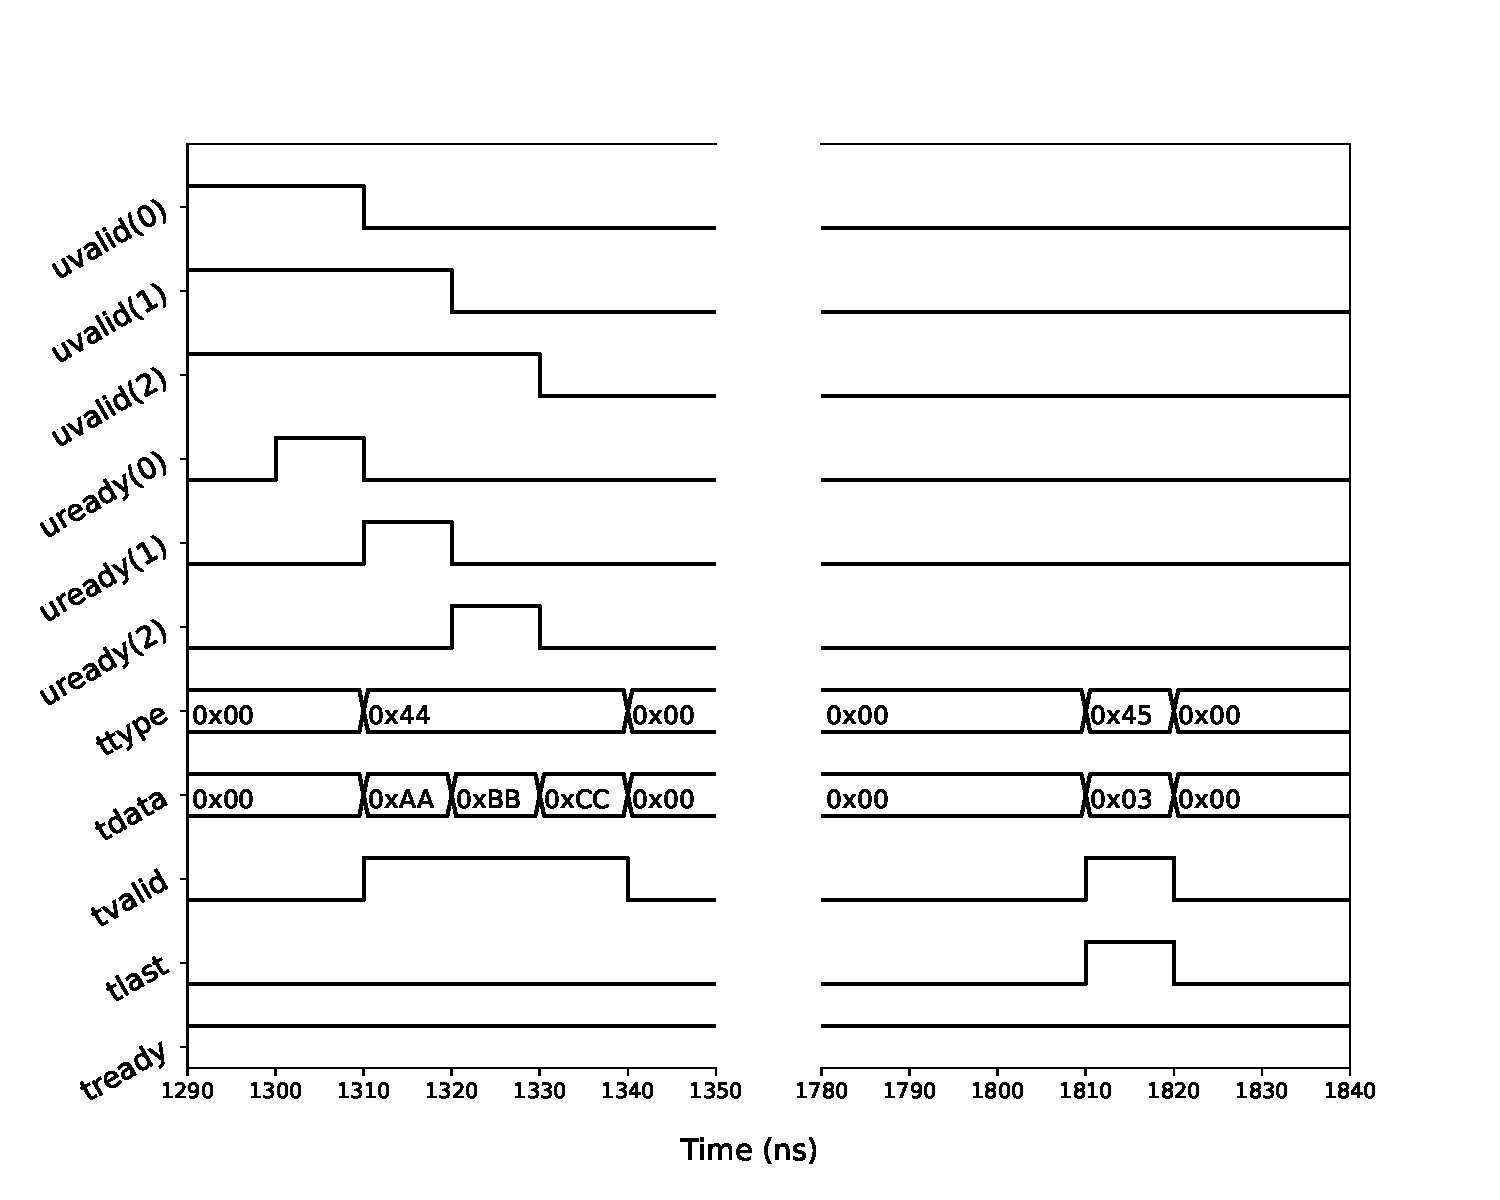
\includegraphics[width=0.85\paperwidth, keepaspectratio]{timing_diagrams/rx_buffer.pdf}
\caption{\label{fig:rx-buffer} RX buffer handling a single DMA packet
  containing data received from three UART channels (output of ghdl
  testbench) For simplicity, only a single indicative byte of the
  stream data (tdata) is shown (e.g. 0xAA).}
\end{figure}

The RX unit uses a valid and ready handshake, as in the AXI protocol,
which was described in previous sections.  Upon receiving a complete
transmission, the RX unit presents the UART data as output and asserts
its UART valid ({\tt uvalid(i)}) signal.  A timing diagram from a GHDL
simulation of the RX buffer operation is presented in
Fig.~\ref{fig:rx-buffer}.  At the start, only UART channels 0-2 have
data available and are each therefore asserting their valid signal.
On the turn assigned to each UART channel, the RX buffer asserts ready
for that channel.  On the next clock cycle, the RX channel deassserts
its valid and the RX buffer presents the data to the stream.  In the
diagram, only an indicative byte of the the stream data is shown, and
in this demonstration UART channel 0 has received 0xAA, channel 1 has
0xBB, and channel 2 has 0xCC, matching the observed pattern.  The
stream data also contains a byte for the word type ({\tt ttype}),
which is 0x44 (the character D in ASCII) for these three UART data
words.  The stream writer asserts stream valid ({\tt tvalid}) for
three clock cycles while these three words are added to the stream.
Since subsequent channels do not have valid data, the stream valid is
deasserted during subsequent turns.

UART data is streamed to the FIFO one word at a time, but multiple
words are assembled into a single DMA packet using the last bit ({\tt
  tlast}) bit.  All data that arrives within a configurable number
(TCYCLES) of turn cycles (64 clock cycles) is included in the same DMA
packet.  In the demonstration of Fig.~\ref{fig:rx-buffer}, the TCYCLES
parameter has been set to 1.  In the second half of the timing
diagram, on turn 50, which occurs 500 ns after the data from channel 0 is placed
in the stream, the stream writer asserts the last ({\tt tlast}) bit,
indicating the end of the packet.  The stream data has its type sent
to END\_OF\_PACKET (0x45 or ASCII character E) and the number of
packets (not including the trailer) 3 is sent.  The indicative byte
was choosen to include this field, so the word count with value 0x3 is
also visible in the diagram.

Upon first seeing data after a pause, the RX buffer does not restart
streaming until the start of the next full cycle (starting at turn 0).
This orders the data in the DMA packet nicely, starting from UART
channel 0, when the data from all UARTs arrives synchronously.

In the demonstration, the FIFO is never full, and so the stream always
asserts stream ready ({\tt tready}).  If the DMA engine were to fall
behind, than the FIFO could fill, and the stream would deassert
stream ready.  This would cause the RX buffer to reframin from asserting any
UART ready ({\tt uready(i)}) signals, which prevents any UART valid ({\tt
  uvalid(i)}) from being cleared.  If new data arrives on any RX channel
before its valid bit is cleared (via ready) the packet is lost, which
is noted by the lost bit in the UART status.  Counters track the
number of lost packets for each UART (which should be always zero
during normal operation).

\begin{table}
\caption{\label{tbl:rx-scope} All RX registers have leading bit 0 and next leading bit 1, and the next six bits define the channel.  That least significant bytes (XX below) further specifies the register.}
\begin{center}
\begin{tabular}{|lll|}
\hline
Channel      & $C$                   & RX Register Address       \\
\hline
UART 0-39    & 0{\rm x}04-0{\rm x}67 & 0{\rm x}40XX-0{\rm x}67XX \\
Broadcast    & 0{\rm x}7B            & 0{\rm x}7BXX              \\
In Common    & 0{\rm x}7F            & 0{\rm x}7FXX              \\
\hline
\end{tabular}
\end{center}
\end{table}

Configuration and monitoring of the RX unit is performed over the
AXI-LITE to REGBUS interface.  In a similar fashion as for the TX
unit, the RX unit is assigned a range of scopes (from 0x4 to 0x7) so
that the most significant byte of the address can be intepreted as:
$${\rm 0b01}cc cccc$$
where
$$C \equiv 0{\rm b}cccccc$$ is the UART channel, taking values from 0 to 63.
As for the TX unit, in addition to the 40 physical UART channels,
assigned channels 0 to 39 (0x00 to 0x27), there are two notional
channels: broadcast (0x3B) and in common (0x3F).  This is summarized
in Table~\ref{tbl:rx-scope}.

\begin{table}
\caption{\label{tbl:rx-reg} Registers managed by the RX unit}
\begin{center}
\begin{tabular}{|llll|}
\hline
Register        & Address   & RWC & Per UART \\
\hline
UART\_STATUS      & 0x00  & RO  & Per UART   \\
UART\_CONFIG      & 0x04  & RW  & Per UART   \\
UART\_LOOK\_A     & 0x10  & RO  & Per UART   \\
UART\_LOOK\_B     & 0x14  & RO  & Per UART   \\
UART\_LOOK\_C     & 0x18  & RO  & Per UART   \\
UART\_LOOK\_D     & 0x1C  & RO  & Per UART   \\
UART\_STARTS      & 0x20  & RO  & Per UART   \\
UART\_BEATS       & 0x24  & RO  & Per UART   \\
UART\_UPDATES     & 0x28  & RO  & Per UART   \\
UART\_LOST        & 0x2C  & RO  & Per UART   \\
UART\_CHAN        & 0x50  & RO  & Per UART   \\
BUFFER\_STATUS    & 0xA0  & RO  & In Common  \\
BUFFER\_CONFIG    & 0xA4  & RW  & In Common  \\
ZERO\_CNTS        & 0xA8  & CMD & In Common  \\
FIFO\_CNT         & 0xB0  & RO  & In Common  \\
FIFO\_MAX         & 0xB4  & RO  & In Common  \\
HEARTBEAT\_CONFIG & 0xC0  & RW  & In Common  \\
ROLLOVER\_CONFIG  & 0xC4  & RW  & In Common  \\
\hline
\end{tabular}
\end{center}
\end{table}


\begin{table}
\caption{\label{tbl:rx-bit-fields} Bit field descriptions for RX register}
\begin{center}
\begin{tabular}{|llll|}
\hline
Register & Field      & Bits & Mask       \\
\hline
UART\_STATUS  & (Expert)   & 31-0  & {\tt 0}x{\tt FFFFFFFF}  \\
\hline
UART\_CONFIG  & RATIO      & 7-0   & {\tt 0}x{\tt 000000FF}  \\
              & PHASE      & 11-8  & {\tt 0}x{\tt 00000F00}  \\
              & MODE       & 13-12 & {\tt 0}x{\tt 00003000}  \\
              & (Reserved) & 15-14 & {\tt 0}x{\tt 0000C000}  \\
              & INPUT      & 17-16 & {\tt 0}x{\tt 00030000}  \\
              & (Reserved) & 31-18 & {\tt 0}x{\tt FFFC0000}  \\
\hline
BUFFER\_STATUS  & (Expert)   & 31-0  & {\tt 0}x{\tt FFFFFFFF}  \\
\hline
BUFFER\_CONFIG  & TCYCLES    & 15-0  & {\tt 0}x{\tt 0000FFFF}  \\
              & (Reserved) & 31-16 & {\tt 0}x{\tt FFFF0000}  \\
\hline
\end{tabular}
\end{center}
\end{table}

The registers managed by the RX unit are presented in
Table~\ref{tbl:rx-reg}, and bit field interpretations for some of the
registers are provided in Table~\ref{tbl:rx-bit-fields}. The UART
configuration (UART\_CONFIG) includes fields for a phase offset (in 10 ns
ticks) and a clock divider (slow down factor) of the RX UART clock
relative to the 100 ns clock sent directly to the ASICs.  Normal
operation is MODE=1.  For MODE=0, the RX unit is squelched: updates
from the UART receivers are ignored, the channel's output is set to
zero, and its valid signal is deasserted.
The RX input is configured by the INPUT parameter.  Normal operation
is INPUT=0 which selects the UART inputs (PISO).  Setting INPUT=1
selects the output of the RX unit for the corresponding channel,
poviding a software loopback option.  Setting INPUT=2 fixes the input
to 0, and INPUT=3 fixes the input to 1.

The RX buffer configuration register (BUFFER\_CONFIG) includes the
TCYCLES field, which specifies the number of turn cycles included in
each DMA packet, as described above.  The sync word behavior is
configured by the number of clock cycles between heartbeats
(HEARTBEAT\_CONFIG) and the timestamp at which a rollover is recorded
(ROLLOVER\_CONFIG).  The UART status registers (USTATUS, one per UART)
and RX buffer status (BSTATUS) interpretation is currently expert
only, and not documented here.

The look registers (UART\_LOOK\_A through and UART\_LOOK\_D) contain the least
significant to most significant 32-bit words (128 bits total) of the
most recent packet received by each packet.  Several counts are
maintained for each UART: the number of start bits received (UART\_STARTS),
beats observed (UART\_BEATS), and successful receptions (UART\_UPDATES).  The
number of lost packets (UART\_LOST), as indicated by the lost bit being
asserted, are likewise counted.  The counts are cleared upon reset and
by writing the zero counts (ZERO\_CNTS) register.  The current number
of words (FIFO\_CNT) in the RX FIFO is available, as is the maximum number
of words (FIFO\_MAX) since the last reset of zero counts command.

\newpage
\subsection{Timing Unit}

The timing unit is reponsible for the 10 MHz clock (UCLK) sent to the
ASICs and producing a timestamp, synchronous with UCLK, which is added
to the incoming data.  The timing unit also handles timing control
signals sent to the ASICs, such as SYNC, RESET, and TRIG signals.  A
fully featured Timing Unit is available in the latest firmware, but we
expect at least one round of substantial revisions before this design
stabalizes, and so we will not document this unit further for this
version.

\subsection{ADC Unit}
The ADC unit is responsible for operating the on-board
high-performance ADC.  A fully featured Timing Unit is available in
the latest firmware, but we expect at least one round of substantial
revisions before this design stabalizes, and so we will not document
this unit further for this version.

%\subsection{Vivado Design and Flow}

\section{PACMAN Server}
\subsection{DAQ Interface}

The PACMAN Server interface to the DAQ is a virtual address spaces.
Virtual addresses refer to specific features, for example, powering
VDDD of tile 1 to a specific voltage level.  The use of a virtual
addresses allows for the most consistent support across hardware
versions.  Direct (non-virtual) interface to the AXI LITE address
space is provided at upper region of the address space, as well as
direct access to the I2C bus.

\begin{table}[htbp]
\centering
\begin{tabular}{|ll|lllll|}
\hline
Word Type & Char & Field & Symbol & Bytes & Bits & Notes \\
\hline
PING  & `P' & PACMAN ID      & P & 1 & 8  & Optional for request\\
\hline
READ  & `R' & PACMAN ID      & P & 1 & 8  & Optional for request\\
~     &     & Address        & A & 4 & 32 & \\
~     &     & Read Value     & R & 4 & 32 & 0 for request\\
\hline
WRITE & `W' & PACMAN ID      & P & 1 & 8  & Optional for request\\
~     &     & Address        & A & 4 & 32 & \\
~     &     & Write Value    & W & 4 & 32 & \\
\hline
DATA  & `D' & PACMAN ID      & P & 1 & 8  & Optional for TX \\
~     &     & Channel        & C & 2 & 16 & \\
~     &     & Timestamp      & T & 8 & 64 & Optional for TX \\
~     &     & Data Payload   & D & 8 & 64 & \\
\hline
CFG   & `C' & PACMAN ID      & P & 1 & 8  & Optional for TX \\
~     &     & Channel        & C & 2 & 16 & \\
~     &     & Timestamp      & T & 8 & 64 & Optional for TX \\
~     &     & Data Payload   & D & 8 & 64 & \\
\hline
SYNC  & `S' & PACMAN ID      & P & 1 & 8  & \\
~     &     & Sync Type      & S & 1 & 8  & \\
~     &     & Clock Sourc    & L & 1 & 8  & \\
~     &     & Timestamp      & T & 8 & 64 & \\
~     &     & Status         & U & 4 & 32 & \\
%\hline
\hline
TRIG  & `T' & PACMAN ID      & P & 1 & 8  & \\
~     &     & Trigger Type   & G & 1 & 8  & \\
~     &     & Trigger Source & I & 1 & 8  & \\
~     &     & Timestamp      & T & 8 & 64 & \\
\hline
ERR   & `E' & PACMAN ID      & P & 1 & 8  & \\
~     &     & Timestamp      & T & 8 & 64 & \\
~     &     & Error Code     & O & 4 & 32 & \\
\hline
\end{tabular}
\caption{Constitutient fields of PACMAN words by word type (with
  associated character).  Each word is 24 bytes (192 bits) but padding
  is not listed here.  The size in bytes (and bits) and the single
  letter symbol used for each active field is listed.}
\label{tbl:pacman_word_fields}
\end{table}

\newcommand{\pacmanWordRect}[1]{%
  % #1 = y-coordinate of the bottom of the rectangle
  \def\wh{1}   % height of the rectangle
  \def\ww{16}   % width of the rectangle
  \def\bw{\ww/24} % width per byte

  % Draw main rectangle
  \draw[line width = 2pt] (0,#1) rectangle (\ww, {#1+\wh});

  % Draw dashed lines for each byte, all relative to #1
  \foreach \i in {1,...,23} {
    \draw[dashed] ({\i*\bw}, #1) -- ({\i*\bw}, {#1+\wh});
  }
}

\newcommand{\pacmanFieldLow}[2]{%
  % #1 = y-coordinate of the bottom of the rectangle
  % #2 = byte index (0..23)
  \def\wh{1}      % height of rectangle
  \def\ww{16}     % width of rectangle
  \def\bw{\ww/24} % width per byte

  % Draw solid line at top of byte #2, relative to bottom y-coordinate #1
  \draw[line width = 2pt] ({#2*\bw}, {#1}) -- ({#2*\bw}, {#1+\wh});
}

\newcommand{\pacmanByteText}[3]{%
  % #1 = y-coordinate of bottom of rectangle
  % #2 = byte index (0–23)
  % #3 = text to place
  \def\wh{1}   % height of rectangle (same as pacmanWordRect)
  \def\ww{16}  % width of rectangle
  \def\bw{\ww/24} % width per byte

  % Compute center of the byte
  \pgfmathsetmacro{\xcenter}{#2*\bw + 0.5*\bw}
  \pgfmathsetmacro{\ycenter}{#1 + 0.5*\wh}

  % Place text centered
  \node at (\xcenter,\ycenter) {#3};
}



\begin{figure}[htbp]
  \centering

  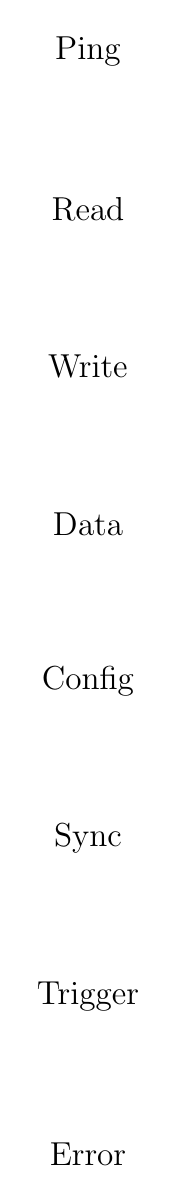
\begin{tikzpicture}
    \def\yERR{0.0}
    \def\yTRIG{2.0}
    \def\ySYNC{4.0}
    \def\yCFG{6.0}
    \def\yDATA{8.0}
    \def\yWRITE{10.0}
    \def\yREAD{12.0}
    \def\yPING{14.0}


    \node at (8,\yPING  - 0.4) {\large Ping};
    \node at (8,\yREAD  - 0.4) {\large Read};
    \node at (8,\yWRITE - 0.4) {\large Write};
    \node at (8,\yDATA  - 0.4) {\large Data};
    \node at (8,\yCFG   - 0.4) {\large Config};
    \node at (8,\ySYNC  - 0.4) {\large Sync};
    \node at (8,\yTRIG  - 0.4) {\large Trigger};
    \node at (8,\yERR   - 0.4) {\large Error};
    
    \pacmanWordRect{\yPING}
    \pacmanByteText{\yPING}{0}{`P'}
    \pacmanFieldLow{\yPING}{1}
    \pacmanByteText{\yPING}{1}{P}
    \pacmanFieldLow{\yPING}{2}

    % READ word
    \pacmanWordRect{\yREAD}
    \pacmanByteText{\yREAD}{0}{`R'}   % word_type
    \pacmanByteText{\yREAD}{1}{P}   % pacman ID
    \pacmanByteText{\yREAD}{8}{A}   % addr
    \pacmanByteText{\yREAD}{12}{V}  % value
    \pacmanFieldLow{\yREAD}{0}    % word_type bottom
    \pacmanFieldLow{\yREAD}{1}    % pacman ID bottom
    \pacmanFieldLow{\yREAD}{2}    % pad(6) bottom
    \pacmanFieldLow{\yREAD}{8}    % addr bottom
    \pacmanFieldLow{\yREAD}{12}   % value bottom
    \pacmanFieldLow{\yREAD}{16}   % pad2(8) bottom

    % WRITE word
    \pacmanWordRect{\yWRITE}
    \pacmanByteText{\yWRITE}{0}{`W'}   % word_type
    \pacmanByteText{\yWRITE}{1}{P}   % pacman ID
    \pacmanByteText{\yWRITE}{8}{A}   % addr
    \pacmanByteText{\yWRITE}{12}{V}  % value
    \pacmanFieldLow{\yWRITE}{0}
    \pacmanFieldLow{\yWRITE}{1}
    \pacmanFieldLow{\yWRITE}{2}    % pad(6)
    \pacmanFieldLow{\yWRITE}{8}
    \pacmanFieldLow{\yWRITE}{12}
    \pacmanFieldLow{\yWRITE}{16}   % pad2(8)

    % DATA word
    \pacmanWordRect{\yDATA}
    \pacmanByteText{\yDATA}{0}{`D'}   % word_type
    \pacmanByteText{\yDATA}{1}{P}   % pacman ID
    \pacmanByteText{\yDATA}{2}{C}   % chan
    \pacmanByteText{\yDATA}{8}{T}   % timestamp
    \pacmanByteText{\yDATA}{16}{D}  % payload
    \pacmanFieldLow{\yDATA}{0}
    \pacmanFieldLow{\yDATA}{1}
    \pacmanFieldLow{\yDATA}{2}
    \pacmanFieldLow{\yDATA}{4}    
    \pacmanFieldLow{\yDATA}{8}
    \pacmanFieldLow{\yDATA}{16}

    % CFG word
    \pacmanWordRect{\yCFG}
    \pacmanByteText{\yCFG}{0}{`C'}   % word_type
    \pacmanByteText{\yCFG}{1}{P}   % pacman ID
    \pacmanByteText{\yCFG}{2}{C}   % chan
    \pacmanByteText{\yCFG}{8}{T}   % timestamp
    \pacmanByteText{\yCFG}{16}{D}  % payload
    \pacmanFieldLow{\yCFG}{0}
    \pacmanFieldLow{\yCFG}{1}
    \pacmanFieldLow{\yCFG}{2}
    \pacmanFieldLow{\yCFG}{4}    
    \pacmanFieldLow{\yCFG}{8}
    \pacmanFieldLow{\yCFG}{16}

    % SYNC word
    \pacmanWordRect{\ySYNC}
    \pacmanByteText{\ySYNC}{0}{`S'}  % word_type
    \pacmanByteText{\ySYNC}{1}{P}  % pacman
    \pacmanByteText{\ySYNC}{2}{S}  % sync_type
    \pacmanByteText{\ySYNC}{3}{C}  % clock_source
    \pacmanByteText{\ySYNC}{8}{T}  % timestamp
    \pacmanByteText{\ySYNC}{16}{S} % status
    \pacmanFieldLow{\ySYNC}{1}   
    \pacmanFieldLow{\ySYNC}{2}   
    \pacmanFieldLow{\ySYNC}{3}   
    \pacmanFieldLow{\ySYNC}{4}   
    \pacmanFieldLow{\ySYNC}{8}   
    \pacmanFieldLow{\ySYNC}{16}  
    \pacmanFieldLow{\ySYNC}{20}  

    % TRIG word
    \pacmanWordRect{\yTRIG}
    \pacmanByteText{\yTRIG}{0}{`T'}  % word type
    \pacmanByteText{\yTRIG}{1}{P}  % pacman
    \pacmanByteText{\yTRIG}{2}{G}  % trigger type 
    \pacmanByteText{\yTRIG}{3}{I}  % trigger source 
    \pacmanByteText{\yTRIG}{8}{T}  % timestamp    
    \pacmanFieldLow{\yTRIG}{1}   
    \pacmanFieldLow{\yTRIG}{2}   
    \pacmanFieldLow{\yTRIG}{3}   
    \pacmanFieldLow{\yTRIG}{4}   
    \pacmanFieldLow{\yTRIG}{8}   
    \pacmanFieldLow{\yTRIG}{16}  

    % ERR word
    \pacmanWordRect{\yERR}
    \pacmanByteText{\yERR}{0}{`E'}  % word type
    \pacmanByteText{\yERR}{1}{P}    % pacman
    \pacmanByteText{\yERR}{8}{T}    % timestamp
    \pacmanByteText{\yERR}{16}{O}   % error code    
    \pacmanFieldLow{\yERR}{1}   
    \pacmanFieldLow{\yERR}{2}   
    \pacmanFieldLow{\yERR}{8}   
    \pacmanFieldLow{\yERR}{16}  
    \pacmanFieldLow{\yERR}{20}  
  \end{tikzpicture}

  \caption{Layout of PACMAN message words by word type, showing field
    locations and sizes, labeled by the single character symbol from
    Table~ \ref{tbl:pacman_word_fields}.  The space between each pair
    of lines represents one byte, and each word is 24 bytes wide
    (192-bits).  The least significant bit is to the left, the the
    least significant byte is a character field used to indicate the
    word type.}
\label{fig:pacman_word_layouts}
\end{figure}

\begin{table}[h]
\centering
\begin{tabular}{|l|l|}
\hline
\textbf{Command} & \textbf{Description} \\
\hline
\texttt{ping}                              & Reply pong \\
\texttt{report\_version\_info}             & Report firmware version and related info \\
\texttt{report\_power}                     & Report voltage and current info  \\
\texttt{read\_pacman\_id}                  & Reply with current PACMAN ID \\
\hline
\texttt{set\_pacman\_id id=<id>}           & Set PACMAN ID to \texttt{<id>} \\
\texttt{set\_vddd tile=<tile> mv=<mv>}     & Set tile \texttt{<tile>} VDDD to \texttt{<mv>}~mV \\
\texttt{set\_vdda tile=<tile> mv=<mv>}     & Set tile \texttt{<tile>} VDDA to \texttt{<mv>}~mV \\
\texttt{enable\_tile\_power}               & Enable main analog power rails for all tiles \\
\texttt{disable\_tile\_power}              & Disable main analog power rails for all tiles \\
\texttt{enable\_tile tile=<tile>}          & Enable local power and logic for tile \texttt{<tile>} \\
\texttt{disable\_tile tile=<tile>}         & Disable local power and logic for tile \texttt{<tile>} \\
\texttt{read\_vddd tile=<tile>}            & Reply with measured VDDD for tile \texttt{<tile>} \\
\texttt{read\_vdda tile=<tile>}            & Reply with measured VDDA for tile \texttt{<tile>} \\
\texttt{read\_enables}                     & Reply with global and per-tile enable status \\
\hline
\texttt{send\_full\_reset mask=<mask>}     & Send full reset to tiles enabled in \texttt{<mask>} \\
\texttt{send\_internal\_reset mask=<mask>} & Send internal reset to tiles enabled in \texttt{<mask>} \\
\texttt{send\_sync\_timestamp mask=<mask>} & Send sync timestamp to tiles enabled in \texttt{<mask>} \\
\hline
\end{tabular}
\caption{High-level DAQ interface commands for the PACMAN card.
All commands use \texttt{key=value} syntax.
Parameters shown in angle brackets (e.g.\ \texttt{<tile>}) indicate user-specified values.
Tile enable operates in two stages: \texttt{enable\_tile\_power} applies global power rails,
and \texttt{enable\_tile} activates individual tiles.}
\label{tbl:high-level}
\end{table}

\newpage
\section{Quality Assurance and Quality Control}

The PACMAN card quality assurance and quality control (QA/QC) regimen
relies on several complementary techniques:
\begin{itemize}

\item {\bf Loopback:} Loopback is generally the most effective method
  of feature verification.  The loopback mindset first drives the
  design toward adequate feedback and test input mechanisms, and then
  tests both the feature and its corresponding feedback or test input
  mechanism simultaneously.  Loopback paths in hardware test
  components and solder quality through the entire path.

\item {\bf Fault Localization:} Designing for fault localization
  forces a modular design that lends itself to effective QC.  For an
  important example, loopback can be performed in the hardware, or in
  firmware (just prior to leaving/ entering the device), or in the
  CPU, so that the source of a failure can immediately be localized to
  hardware, programmable logic, or software.

\item {\bf Design Review:} The PACMAN design team includes a lead
  engineer, and a consulting engineer, and a principile investigator.
  All three understand the board down to the last net list.  The
  PACMAN design is also periodically subjected to independent review.

\item {\bf Prototype Systems:} The most effective form of quality
  control is operation in a working system, and the PACMAN card has
  been used continuously in prototype systems since the first version
  in 2020.

\end{itemize}

\subsection{Feature Verification Overview}

Here we list design features of the PACMAN card that are tested during
hardware verification, in most cases by a loopback mechanism.
Specific details on performing the relevant tests are discussed in the
hardware checkout section.
\begin{itemize}
\item The LEDs are tested with blink patterns.

\item The provision of tile voltages VDDD and VDDA is verified by
  onboard current and voltage monitoring ADCs.

\item The POSI and PISO (Digital I/O to Tiles) signals are tested via
  loopback using both test patterns and pseudorandom numbers.

\item The onboard high-performance ADC is tested by connecting both
  the positive and negative terminals to independently controlled DAC
  outputs.

\item The CLK, RESETN/SYNC/TRIG signals (Digital I/O to Tiles) are
  tested by loopback to the onboard ADC (DONE) through the ASIC
  Monitoring Channels.  In addition to these signals, this therefore
  tests MUX and the Analog Monitoring Signals.

\item The CLK, RESETN/SYNC/TRIG signals (Digital I/O to Tiles) are
  tested by loopback to PISO channels (Not yet implemented, test above
  suffices).

\item The Front-Panel SMA connectors and MUX are checked by leaving
  them open or connecting a resistor in software and confirming the
  resistance with a DMM (Not yet in Linux)

\item The Front-Panel LEMO connectors are checked by driving them with
  external TTL signals and checking counters in the software.

\end{itemize}

The PACMAN card hosts a linux system, so a broad spectrum of test
software is immediately available to us.  Here we list what we
consider to the be the most important tests of the Linux host.
Specific details on performing the relevant tests are discussed in the
hardware checkout section.

\begin{itemize}
\item Successful system BOOT, visible via UART.
\item Successful remote login via ethernet.
\item Successful transfer of psuedo-random data via ethernet (scp) and the UART terminal (lrzsz).
\item Repeated read and write of psuedo-random numbers to the SD card.
\end{itemize}

Some of the tests described in this section require configuring the
PACMAN card in ways that are not appropriate for a card installed in
the production system.  For this reason, the PACMAN card includes an
expert mode enable two pin jumper.  When a PACMAN card is installed in
the production system, this jumper is removed, and the software
refuses to provide inappropriate test configurations.

\subsection{Requirement Verification}

In addition to feature operation, the PACMAN has several performance
requirements which require quantitative verifications:

\begin{itemize}
 \item The provision of voltage and power across the required ranges
   is tested by applying the appropriate load resistance to VDDD and VDDA.
 \item The common mode rejection feature of the DC voltage supply is
   tested by injecting larger than expected common mode noise at the
   input and measuring the provided DC voltage (This test will be performed on a subset of the PACMAN cards, to validate the design.)
 \item The bit error rate is measured during loopback testing of the digital I/O systems.
 \item The high-frequency noise rejection is tested by injecting a
   high-frequency signal at the input and measuring the signals after
   filtering. (This test will be performed on a subset of the PACMAN cards, to validate the design)
 \item Temperature dependence (TBD)
 \item Limits of digital I/O (clock speed, long cables) (TBD)
\end{itemize}

\section{Hardware Checkout Proceedure}

Caveats: No allowed tolerances have been provided yet, because we have
only tested a few boards.

\subsection{Bare Board}

\begin{center}
\begin{tabular}{cc}
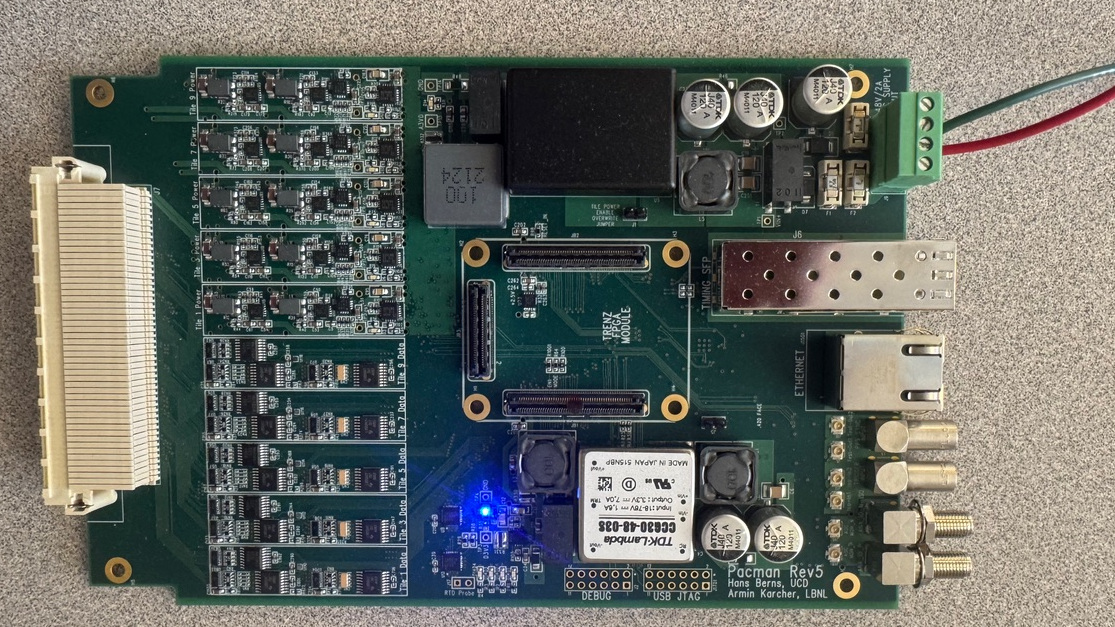
\includegraphics[height=0.26\textwidth]{photos/bare_one_led.jpeg} &
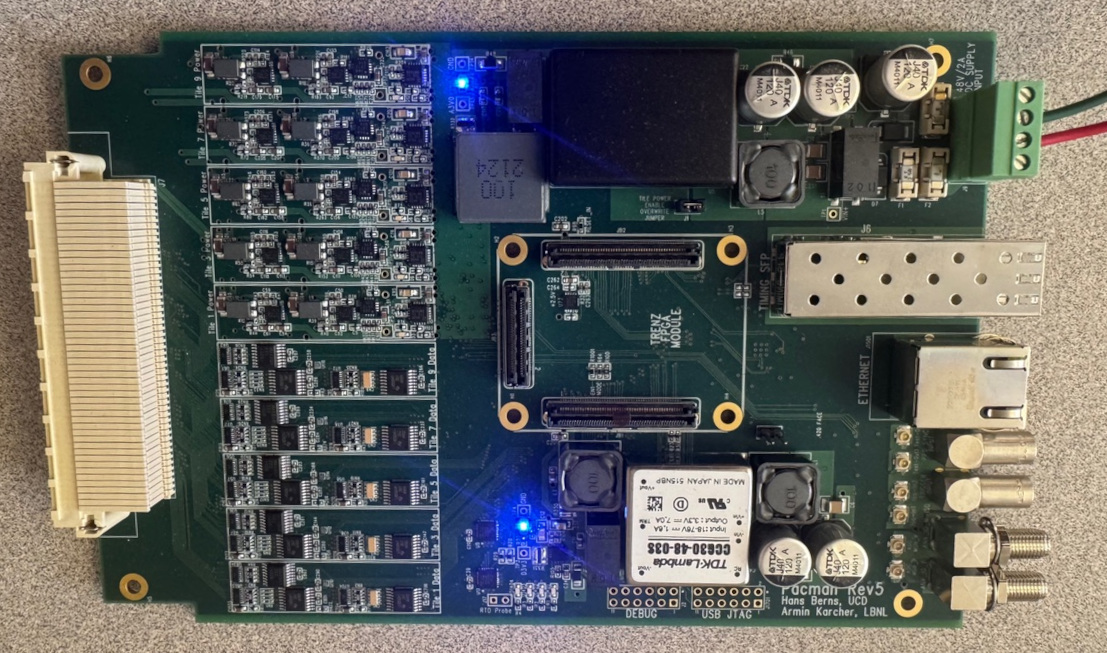
\includegraphics[height=0.26\textwidth]{photos/bare_two_led.jpeg} \\
Board Power Only & Tile Power Enabled (jumper)

\end{tabular}
\end{center}

The hardware checkout begins with a bare board (no TRENZ module
installed).  The $3.3\rm V$ digital power (used by PACMAN) is on as
soon as the board is powered at the DC supply input.  The board also
includes a jumper ``TILE POWER ENABLE OVERRIDE JUMPER'' which allows
the 3.3~\rm V tile power to be validated before installing any module.

The current should be measured and compared to the nominal expected
value for the applied voltage, in the range of positive $32~\rm V$ to
positive $48~\rm V$):
\begin{center}
\begin{tabular}{|l|l|l|l|}
\hline
Voltage (V) & Current (mA)  &  Current (mA) \\
            & (No Jumper)   & (Analog Power Enabled) \\
48          & 66            & 100 \\
40          & 77            & 113 \\
36          & 91            & 131 \\
\hline
\end{tabular}
\end{center}

Using a DMM, verify the supply of 3.3 V (nominal) at TP3 (D3V3) relative to TP4 (GND).

Using a DMM, verify the supply of 3.0 V (nominal) at TP13 (A3V0) relative to TP14 (GND).

\subsection{TENZ Module and Linux System Checks}

With a TRENZ module installed on the board, insert an SD card with the
latest hardware checkout firmware, the ethernet cable connected to the
network, and power the board.

The local network may require customizations to the ROOT filesystem in
order to bring up the ethernet connection.  Before attempting to bring
up the network on a headless PACMAN card (no USB JTAG/UART header has
been installed) consider debuging the network configuration on a
PACMAN equipped with a USB JTA/UART header or a Trenz Module ...  Once
the network is brought up reliably, you can boot a PACMAN with no
terminal and connect over ethernet.

Login to the pacman card via ethernet.

Run the following Linux diagnostic tools (TBD).

The Linux-based drivers depend the Linux GPIO interface in /sys/class.
This should be initialized at boot via the gpio\_init script included
with the hwutil package.  Confirm that this is working properly with:
\begin{lstlisting}[language=sh,frame=leftline]
root@Trenz:~# ls /sys/class/gpio/
export	gpio906  gpio913  gpio918  gpio919  gpiochip906  unexport
\end{lstlisting}

\subsection{Linux-based Hardware Checkout Application}

The PACMAN hardware demonstration firmware includes a menu interface to the Linux drivers:  pacman\_menu.  It is available from the command line as:
\begin{lstlisting}[language=sh,frame=leftline]
root@Trenz:~# pacman_menu
pacman_menu:  PACMAN Linux driver access via menu, for diagnostics and hardware checkout.
INFO:  Opening /dev/mem.
INFO:  Initializing PACMAN AXI-Lite interface.
INFO:  Running pacman firmware version 3.2 (Build: 0x7fff0000  HW Code:  0x10500)
INFO:  Opening /dev/mem.
INFO:  Initializing PACMAN BRAM (AXI-LITE) interface.
INFO:  Opening /dev/mem.
INFO:  Initializing DMA contol interface (AXIL).
INFO:  Initializing DMA TX_BUFFER.
INFO:  Initializing DMA RX_BUFFER.
MAIN MENU:  choose an option:
(1) blink LEDs (2) global registers (3) toggle scratch registers
(4) power menu (5) RX/TX menu (6) timing menu (7) ADC menu
\end{lstlisting}
The user selects menu options by typing the number for the option
followed by enter.  The numbers and arrangement of the menu's will
vary with firmware version as we further develop the tools.  This
documentation is based on hardware demonstration firmware version 3.2.
In the future, we will support a turn-key hardware checkout routine as
a menu option.  However, here we document each individual test
one-by-one.

\subsubsection{LED checkout}

The pacman\_menu can be used to blink the LEDs as follows:
\begin{lstlisting}[language=sh,frame=leftline]
MAIN MENU:  choose an option:
(1) blink LEDs (2) global registers (3) toggle scratch registers
(4) power menu (5) RX/TX menu (6) timing menu (7) ADC menu
1
INFO: selected 1
INFO: starting LED blink test...
Blinking RED LED on Trenz Module, via MIO...
Blinking PACMAN LED-0, via MIO...
Blinking PACMAN LED-1, via MIO...
Blinking PACMAN LED-2, via AXIL register...
Blinking PACMAN LED-3, via AXIL register...
INFO: done with LED blink test.
MAIN MENU:  choose an option:
(1) blink LEDs (2) global registers (3) toggle scratch registers
(4) power menu (5) RX/TX menu (6) timing menu (7) ADC menu
\end{lstlisting}
The user should verify that:
\begin{itemize}
\item The red LED on the TRENZ module blinks
\item The four green LEDs on the PACMAN card blink one-by-one.
\end{itemize}
This simple test also confirms that the MIO and AXI-Lite register interfaces are both working.

\subsubsection{Board Power}
Control and monitoring of electrical power provided by the PACMAN is accessible from the power menu:
\begin{lstlisting}[language=sh,frame=leftline]
MAIN MENU:  choose an option:
(1) blink LEDs (2) global registers (3) toggle scratch registers
(4) power menu (5) RX/TX menu (6) timing menu (7) ADC menu
4
INFO: selected 4
POWER MENU:  choose an option:
(0) main menu (1) toggle enables (2) toggle power (3) monitor power
(4) write IV curves to file
\end{lstlisting}

The ``toggle enables'' feature steps through various combinations of
the Tile Power Enable\footnote{Also called ``Analog Power Enable'' but
this is misleading as it provides both digital and analog power to the
tile cards.} and the ten individual Tile enables.  The accessible settings include:\\[5pt]
\begin{tabular}{ll}
Setting & Explanation \\
\hline
0x00000000 & Nothing Enabled \\
0x00010000 & Tile Power enabled, no individual Tiles enabled\\
0x00010001 & Tile Power enabled, only Tile 1 enabled\\
0x000103FF & Tile Power enabled, all Tiles enabled\\
\end{tabular}{ll}\\[5pt]
The ``monitor power'' feature access the on-board voltage and current monitoring ADCs.  At the moment, we are only concerned with the Board Power monitoring:
\begin{lstlisting}[language=sh,frame=leftline]
BOARD POWER SUMMARY:
Board 3V6:  voltage:   3526 mV  current:   1337 mA
Board 3V3:  voltage:   3326 mV  current:    813 mA
Board 3V0:  voltage:   2985 mV  current:      0 mA
\end{lstlisting}
The user should verify that:
\begin{itemize}
\item As you step through the enables, first the Tile Power Enabled LED lights, then the Tile 1 enable LED lights, then all the Tile enable LEDs light.
\item The Board 3V0 voltage is near either $3000~\rm mV$ or zero depending on whether the TILE Power is enabled or not.
\item (The RTD Probe feature can be tested here as well by connecting a resistor at J17)
\end{itemize}

\subsubsection{VDDD and VDDDA}

The ``write IV curves to file'' feature of the Power submenu steps
through several different DAC settings and steps through the monitored
values of the voltages VDDA and VDDD along with the corresponding
currents IDDA and IDDD.  The collected data (saved as a text file) can
be plotted to show the linearity of the provided voltage with DAC
setting, and the IV curve for each supplied voltage.
\begin{center}
\begin{tabular}{cc}
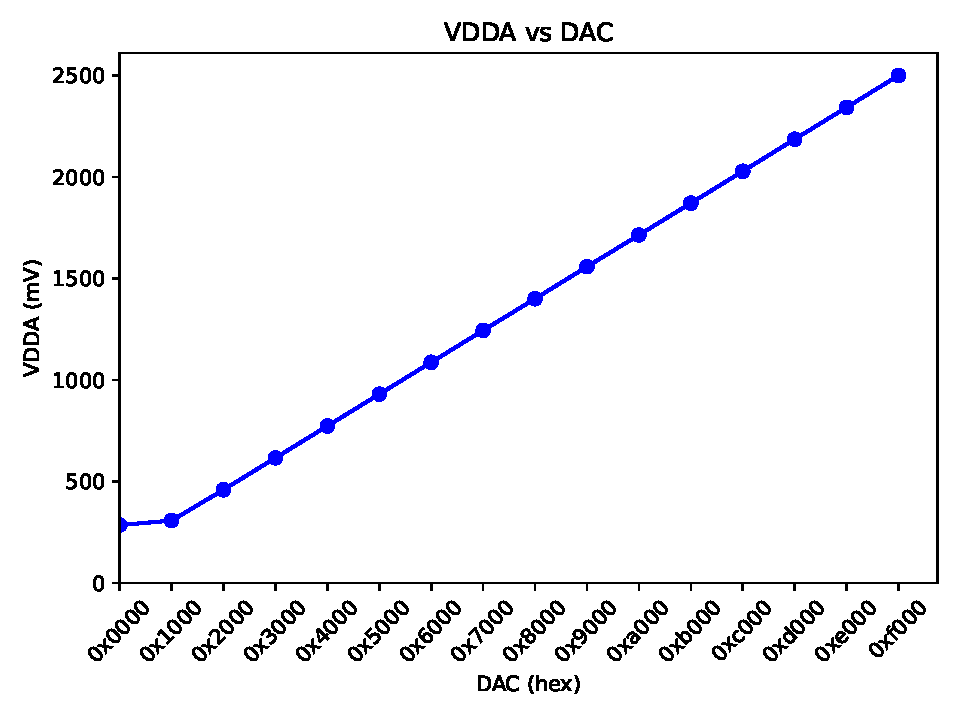
\includegraphics[height=0.36\textwidth]{plots/vdda_dac.pdf} &
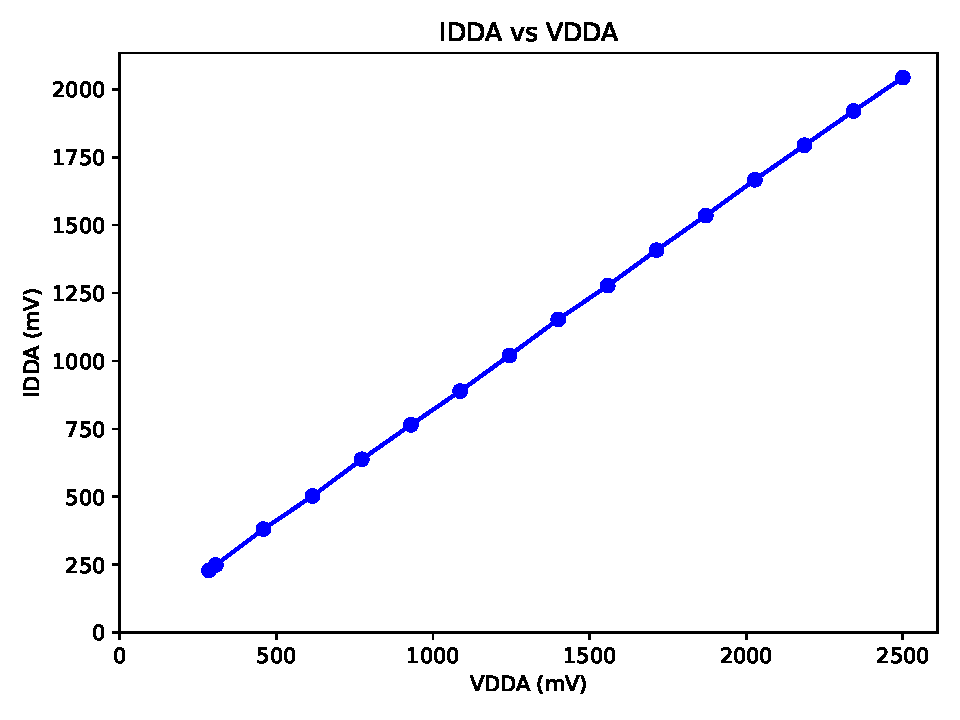
\includegraphics[height=0.36\textwidth]{plots/idda_vdda.pdf} \\
\end{tabular}
\end{center}
Here the VDDA has been loaded with a resistor to ground at the
loopback card.

\subsubsection{POSI/PISO Loopback Testing with Random Numbers}

One of the most important checks is the RX and TX capabilities for the
POSI and PISO signals between the PACMAN and the LArPix ASICs.  We
test these with loopback at twice the nominal ASIC clock rate.  We
transmit known random values out of the PACMAN, physically loop them
back in as inputs.  We check each received word against the random
value that was sent.  This test is available through the RX/TX
submenu, but requires a few steps:
\begin{itemize}
\item Set the global RX configuration to 0x00000001.  This disables heartbeat, sync, and trigger words which could confuse the test.  It also only includes a single cycle in each transmitted DMA buffer.
\item Set RX configuration to 0x00001001. This sets the mode to 1 (normal operation) and full speed (clock divisor 1).
\item Set TX configuration to 0x00001601. This sets the mode to 1 (normal operation), phase to 0x60, and full speed (clock divisor 1).
\item Stop pacman\_server (both the data server and command server) via:
\begin{lstlisting}[language=sh,frame=leftline]
root@Trenz:~# pacman_server stop
Stopping command server...
Stopping dataserver...
\end{lstlisting}
It is most convenient if you wait to do this until after the global RX configuration has been set to disables heartbeat, sync, and trigger words.  That way, the pacman\_cmdserver drains the FIFO.
\item Stopping pacman\_cmdserver leaves a pending DMA read request, so either reset DMA, or sent a single RX.  When ready for the test, a single TX leaves the fifo size at 37 (40 + 1 128 bit words minus four words buffered by the vendor supplied DMA engine) which should be read by a single RX, leaving the fifo size at 0.
\end{itemize}
Once preparations are complete, the test is easily run:
\begin{lstlisting}[language=sh,frame=leftline]
RX/TX MENU:  choose an option:
(0) main menu (1) zero counts (2) toggle TX config (3) toggle RX config (4) toggle RX global config
(5) TX status  (6) TX look   (7) single TX
(8) RX status  (9) RX look   (10) single RX
(11) benchmark TX  (12) benchmark RX/TX loopback (13) random RX/TX loopback
(14) DMA status (15) reset DMA
(16) set DMA TX to RUN
(17) set DMA RX to RUN (18) clear DMA RX (19) start DMA RX (20) resume RX
13
INFO: selected 13
INFO:  Setting DMA TX To RUN.
INFO:  DMA TX has left the HALTED state successfully. (timeout=100)
INFO:  Setting DMA RX To RUN.
INFO:  DMA RX has left the HALTED state successfully. (timeout=100)
SUMMARY: Found 0 discrepancies in 40000 uart packets
\end{lstlisting}

The user should verify that:
\begin{itemize}
\item The test can be run several times with zero discrepancies detected.
\end{itemize}
Note that to help distinguish hardware failures from software
failures, you can configure internal loopback mode (so that loopback
occurs in software not hardware).

\subsubsection{Clock and Reset/Sync/Trigger Signals}

To test the Clock and Reset/Sync/Trigger signals, these are routed
back to PACMAN via loopback into the analog monitoring signals.  These
can be directed to the ADC, which acts as a digital oscilloscope to
record the waveforms:
\begin{center}
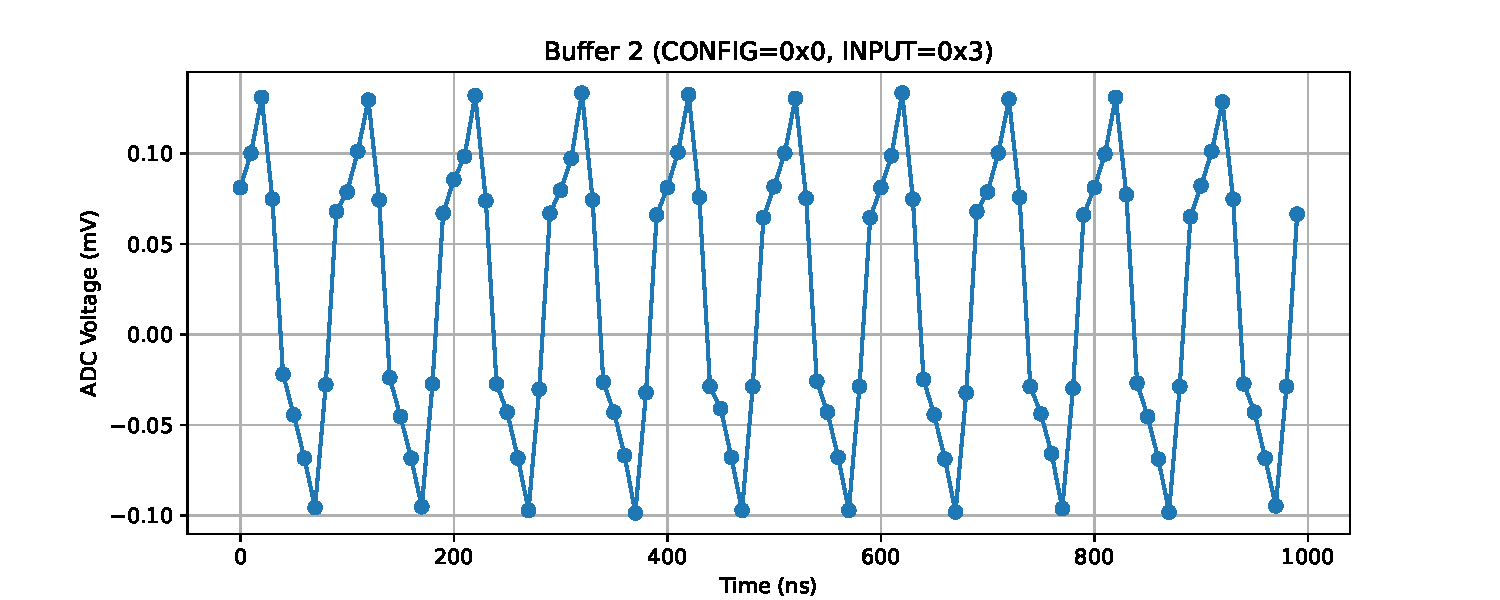
\includegraphics[height=0.36\textwidth]{plots/clock.pdf}\\
\end{center}

\begin{center}
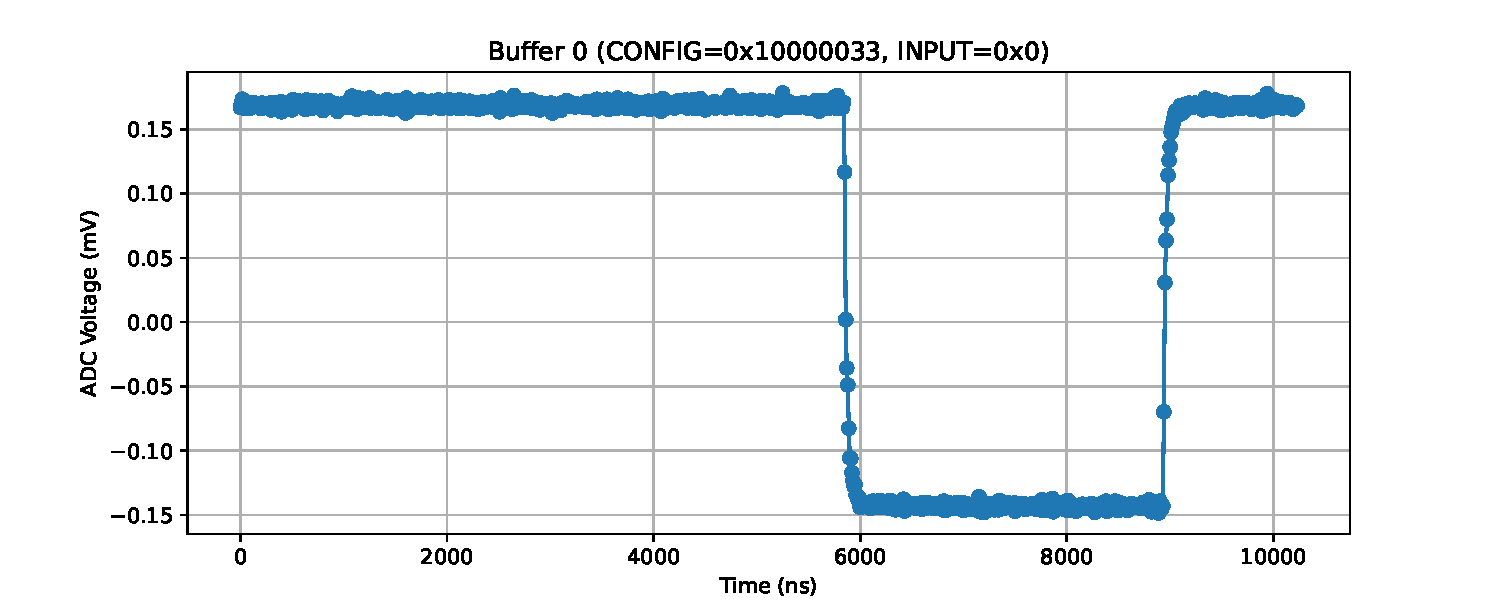
\includegraphics[height=0.36\textwidth]{plots/timing.pdf}\\
\end{center}


\subsubsection{Front Panel Checkout}
\begin{itemize}
\item (the MUX can be adjusted to provide a 100 Ohm resistance, or open
 circuit, between the two SMA connectors, which can be verified with a
 DMM.)
\item (the TTL pulses can be fed into the LEMO connectors, which are counted by the timing unit, with counts available from the timing sub-meno.)
\end{itemize}

\appendix

\section{Specifications for the PACMAN Card}

\subsection{Overview}

Each PACMAN card provides power, digital I/O, and analog test and
monitoring signals to up to ten pixel tile cards.  Each pixel tile
card will consist of 160 ASICs (CONFIRM).

\subsection{Power}

The PACMAN card provides digital and analog power to up to ten pixel
tile cards.  The digital voltage level (VDDD) and analog voltage level
(VDDA) are digitally controlled independently for each pixel tile
card, within the limits and at the stability specified below.

The power requirements of the PACMAN are based on scaling the measured
power consumption of the 100 ASIC pixel tile cards to 160 ASIC pixel
tile cards of the production system, a scale factor of 1.6.  An
additional (minimum) safety factor of $10\%$ is added to these
extrapolated power requirements to derive the following
specifications:
\captionof{table}{Digital and Analog Power Requirements (per tile card)}
\begin{center}
\begin{tabular}{llllll}
      & Stability & Min (V) & Max (V) & Max Current (A) & Max Power (W) \\
VDDA  & $1\%$ & 0 & 1.8 & 0.3 & 0.7\\
VDDD  & $1\%$ & 0 & 1.8 & 1.1 & 2.2\\
\end{tabular}
\end{center}

Reaching a $1\%$ stability on VDDA and VDDD requires linear regulation
and so the power requirements at the input of the PACMAN are derived
from a higher voltage level of $3~\rm V$.  This implies that the
initial switching voltage requirement must provide at least 42 W at
$3~\rm V$.

The PACMAN power is provided by a single nominal 48~V 2~A DC input.
The power connection is the four position terminal connector (Phenoix
Contact P/N 5444660).  The inner two pins provide power and the outer
two are for sense: \captionof{table}{Input Power Connections}
\begin{tabular}{ll}
pin & function \\
1 & V+ sense  \\
2 & V+ \\
3 & V- \\
4 & V- sense \\
\end{tabular}\\
The connector is rated for 8 A and 300 V.  The PACMAN is fused at 2.5
A and has over voltage protection at 60 V.  The sense pins are fused
at 0.5 A.

\subsection{Digital Signals}

The LArPix-v2 ASIC uses a bit-serial protocol to transmit and receive
data.  The PACMAN is the primary and the LARPix ASIC the secondary, so
that the PACMAN transmits POSI and receives PISO signals.

The PACMAN shall provide the following digital IO signals to each
pixel tile card:
\captionof{table}{Digital Signals (per pixel tile card)}
\begin{center}
\begin{tabular}{llllll}
Signal & Quantity & Description \\
  POSI & 4 & Bit serial transmission to pixel tile \\
  PISO & 4 & Bit serial reception from pixel tile \\
  CLK  & 1 & Clock \\
  TRIG & 1 & Trigger \\
  SYNC & 1 & Multiplexed Synchronization and Reset \\
\end{tabular}
\end{center}

Each POSI signal is received by a single ASIC, but the clock, trigger,
and sync signals are fanned out to every ASIC on the tile card.  The
PACMAN must be capable of driving the resulting capacitive load.

The nominal clock rate is $10~\rm MHz$ with a maximum of $40~\rm MHz$.
The LArPix ASIC uses an LVDS signal with custom voltage level which
the PACMAN is capable of transmitting and receiving.

\subsection{Noise}

The noise injected into the pixel tile from the controller is less than $1~\rm mV$.

\subsection{Pixel Tile Interface}

A single PACMAN card drive up to ten pixel tile cards through a single
flange card.  The interface to the eight-tile flange card is through a
6 row by 50 pin high-desnity SAMTEC connector {\tt
  SEAF-50-01-L-06-1-RA-K-TR} on the PACMAN card.

The PACMAN card shall provide a footprint for an optional 2x17
connector to drive a pixel card directly without the use of flange
card.

\subsection{Front Panel Interface}

The PACMAN card implements the front-panel interfaces listed below in
the specified quantity with specified routing.  When routing to
programmable logic (PL) is specified, the specified purpose is nominal
and can be repurposed through firmware changes.

\captionof{table}{Required Front Panel Interface}
\begin{center}
\begin{tabular}{lll}
Interface   & Quantity & Routing \\
SMA Jack    & 1 & Multiplexed to eight tile analog monitor \\
SMA Jack    & 1 & Multiplexed to eight tile adc test \\
Lemo Jack   & 2 & PL: Trigger and Sync \\
Push Button & 1 & Reset \\
LED         & 4 & PL: General Purpose
\end{tabular}
\end{center}


\subsection{Timing System Endpoint}

The PACMAN card implement a ProtoDUNE-SP timing system
endpoint\footnote{DUNE-doc-1651-v3} of a single fiber-optic link.

\subsection{Embedded Linux}

The PACMAN is an embedded Linux system and supports several standard embedded Linux interfaces:\\
\begin{tabular}{lll}
Interface & P/N & Notes \\
Ethernet & & Gigabit \\
SD Card & & Bootable from SD card\\
JTAG & & SoC Configuration\\
UART & & Linux Terminal\\
\end{tabular}\\
The JTAG and UART interface are multiplexed to provide a linux terminal and firmware configuration over a single USB port.


\newpage
\section{PACMAN Version History}

\captionof{table}{PACMAN Evolution}
\vskip 0.5cm
\begin{center}
\begin{tabular}{llll}
Card        & Designer      & Date & Notes \\
\hline
PACMAN 1v1  & Hillbrand      & Feb 2020  & Initial Prototype (Not Supported) \\
PACMAN 1v2  & Karcher        & July 2020 & Single-tile capable (Not Supported) \\
PACMAN 1v3  & Berns/Karcher  & Jan 2021  & Eight-tile capable - Module 0\\
PACMAN 1v4  & Berns/Karcher  & Feb 2022  & LArPix-v2b, Power, TX\\
PACMAN 1v5  & Berns/Karcher  & Aug 2024  & Ten-tile capable \\
PACMAN 1v5b & Berns/Karcher  & TBD 2025  & Interchangeable w/ 1v5\\
\end{tabular}
\end{center}

\section{Prototype Results}

Many of the specifications for the PACMAN are driven by measurements,
using prototype devices, as described in this section.

The Intrinsic RMS noise on the LArPix ASIC was
benchtested\footnote{Reported 6 Mar 2020, Brooke} at $~\sim 3~\rm mV$.

The PACMAN card provides digital (VDDD) and analog (VDDA) power for
the LArPix ASICs.  The ASIC power draw during power up was
measured\footnote{Reported 13 Feb 2020, Brooke} as follows:
\captionof{table}{ASIC Current Draw at Power-up}
\begin{center}
\begin{tabular}{lllll}
   & Voltage (V) & Current (mA) & Power (mW) & Power ($\rm \mu W / chan$)\\
VDDA  & 1.8 & 1.4  & 2.5  & 39\\
VDDD  & 1.8 & 6.92 & 12.5 & 195\\
\end{tabular}
\end{center}

\newpage
The 10x10 pixel-tile power draw was measured \footnote{Reported 14 Jan 2021, Brooke} as follows:
\captionof{table}{10x10 Power Draw}
\begin{center}
\begin{tabular}{llll}
   & Voltage (V) & Current (mA) & Power (W) \\
VDDA  & 1.8 & 166  & 0.3  \\
VDDD  & 1.8 & 611  & 1.1  \\
\end{tabular}
\end{center}


\end{document}
